\newcommand{\model}{Anritsu MS46322A}

\documentclass[12pt,openany,a4paper]{book}
\newcommand\tabSpace[1][1cm]{\hspace*{#1}}
\usepackage{graphicx}
\usepackage{ragged2e}
\usepackage{enumitem}
\usepackage{listings}
\usepackage{amsmath}
\usepackage{color} 
\usepackage{float}
\usepackage{pdflscape}
\usepackage{multirow}
\usepackage{longtable}
\usepackage[subnum]{cases}
\usepackage{caption}
\usepackage{tabularx} % in the preamble

%Code coloring
\usepackage{color}
\definecolor{dkgreen}{rgb}{0,0.6,0}
\definecolor{gray}{rgb}{0.5,0.5,0.5}
\definecolor{mauve}{rgb}{0.58,0,0.82}
\lstset{
  language=C,
  xleftmargin=\parindent,
  aboveskip=3mm,
  belowskip=3mm,
  showstringspaces=false,
  columns=flexible,
  basicstyle={\small\ttfamily},
  numbers=left,
  numberstyle=\tiny\color{gray},
  keywordstyle=\color{blue},
  commentstyle=\color{dkgreen},
  stringstyle=\color{mauve},
  breaklines=true,
  breakatwhitespace=true,
  tabsize=3
}

%BibTeX referencing packages
\usepackage{lmodern}
\usepackage{hyperref}
%\usepackage{breakurl}

\newcolumntype{L}[1]{>{\raggedright\let\newline\\\arraybackslash\hspace{0pt}}m{#1}}
\newcolumntype{C}[1]{>{\centering\let\newline\\\arraybackslash\hspace{0pt}}m{#1}}
\newcolumntype{R}[1]{>{\raggedleft\let\newline\\\arraybackslash\hspace{0pt}}m{#1}}



% If you use a macro file called macros.tex :
% \input{macros}
% Note: The present document has its macros built in.

% Number subsections but not subsubsections:
\setcounter{secnumdepth}{2}
% Show subsections but not subsubsections in table of contents:
\setcounter{tocdepth}{2}

\pagestyle{headings}		% Chapter on left page, Section on right.
\raggedbottom

\setlength{\topmargin}		{-5mm}  %  25-5 = 20mm
%\setlength{\oddsidemargin}	{10mm}  % rhs page inner margin = 25+10mm
\setlength{\oddsidemargin}	{0mm}  % CHANGED THIS BECAUSE I DIDNT LIKE IT
\setlength{\evensidemargin}	{0mm}   % lhs page outer margin = 25mm
\setlength{\textwidth}		{150mm} % 35 + 150 + 25 = 210mm
\setlength{\textheight}		{240mm} % 

\renewcommand{\baselinestretch}{1.2}	% Looks like 1.5 spacing.

% Stop figure/tables smaller than 3/4 page from appearing alone on a page:
\renewcommand{\textfraction}{0.25}
\renewcommand{\topfraction}{0.75}
\renewcommand{\bottomfraction}{0.75}
\renewcommand{\floatpagefraction}{0.75}

% THEOREM-LIKE ENVIRONMENTS:
\newtheorem{defn}	{Definition}	% cf. \dfn for cross-referencing
\newtheorem{theorem}	{Theorem}	% cf. \thrm for cross-referencing
\newtheorem{lemma}	{Lemma}		% cf. \lem for cross-referencing

% AIDS TO CROSS-REFERENCING (All take a label as argument):
\newcommand{\eref}[1] {(\ref{#1})}		% (...)
\newcommand{\eq}[1]   {Equation~(\ref{#1})}		% Eq.~(...)
\newcommand{\eqs}[2]  {Eqs.~(\ref{#1}) and~(\ref{#2})}
\newcommand{\dfn}[1]  {Definition~\ref{#1}}	% Definition~...
\newcommand{\thrm}[1] {Theorem~\ref{#1}}	% Theorem~...
\newcommand{\lem}[1]  {Lemma~\ref{#1}}		% Lemma~...
\newcommand{\fig}[1]  {Figure~\ref{#1}}		% Fig.~...
\newcommand{\tab}[1]  {Table~\ref{#1}}		% Table~...
\newcommand{\chap}[1] {Chapter~\ref{#1}}	% Chapter~...
\newcommand{\secn}[1] {Section~\ref{#1}}	% Section~...
\newcommand{\ssec}[1] {Subsection~\ref{#1}}	% Subsection~...

% AIDS TO FORMATTING:
\newcommand{\teq}[1]	{\mbox{$#1$}}	% in-Text EQuation (unbreakable)
\newcommand{\qed}	{\hspace*{\fill}$\bullet$}	% end of proof

% MATHEMATICAL TEMPLATES:
% Text or math mode:
\newcommand{\half}	{\ensuremath{\frac{1}{2}}}	% one-half
\newcommand{\halftxt}	{\mbox{$\frac{1}{2}$}}	  	% one-half, small
% Math mode only:
% N.B. Parentheses are ROUND; brackets are SQUARE!
\newcommand{\oneon}[1]	{\frac{1}{#1}}		  % reciprocal
\newcommand{\pow}[2]	{\left({#1}\right)^{#2}}  % Parenthesized pOWer
\newcommand{\bow}[2]	{\left[{#1}\right]^{#2}}  % Bracketed pOWer
\newcommand{\evalat}[2]	{\left.{#1}\right|_{#2}}  % EVALuated AT with bar
\newcommand{\bevalat}[2]{\left[{#1}\right]_{#2}}  % Bracketed EVALuated AT
% Total derivatives:
\newcommand{\sdd}[2]	{\frac{d{#1}}{d{#2}}}		    % Short
\newcommand{\sqdd}[2]	{\frac{d^2{#1}}{d{#2}^2}}	    % 2nd ("SQuared")
\newcommand{\ldd}[2]	{\frac{d}{d{#1}}\left({#2}\right)}  % Long paren'ed
\newcommand{\bdd}[2]	{\frac{d}{d{#2}}\left[{#2}\right]}  % long Bracketed
% Partial derivatives (same sequence as for total derivatives):
\newcommand{\sdada}[2]	{\frac{\partial {#1}}{\partial {#2}}}
\newcommand{\sqdada}[2]	{\frac{\partial ^{2}{#1}}{\partial {#2}^{2}}}
\newcommand{\ldada}[2]	{\frac{\partial}{\partial {#1}}\left({#2}\right)}
\newcommand{\bdada}[2]	{\frac{\partial}{\partial {#1}}\left[{#2}\right]}
\newcommand{\da}	{\partial}

% ORDINAL NUMBERS:
\newcommand{\ith}	{\ensuremath{i^{\rm th}}}
\newcommand{\jth}	{\ensuremath{j^{\rm th}}}
\newcommand{\kth}	{\ensuremath{k^{\rm th}}}
\newcommand{\lth}	{\ensuremath{l^{\rm th}}}
\newcommand{\mth}	{\ensuremath{m^{\rm th}}}
\newcommand{\nth}	{\ensuremath{n^{\rm th}}}

% SINUSOIDAL TIME AND SPACE-DEPENDENCY FACTORS:
\newcommand{\ejot}	{\ensuremath{e^{j\omega t}}}
\newcommand{\emjot}	{\ensuremath{e^{-j\omega t}}}

% UNITS (TEXT OR MATH MODE, WITH LEADING PADDING SPACE IF APPLICABLE):
% NB: These have not been tested since being modified for LaTeX2e.
\newcommand{\pack}	{\hspace{-0.08em}}
\newcommand{\Pack}	{\hspace{-0.12em}}
\newcommand{\mA}	{\ensuremath{\rm\,m\pack A}}
\newcommand{\dB}	{\ensuremath{\rm\,d\pack B}}
\newcommand{\dBm}	{\ensuremath{\rm\,d\pack B\pack m}}
\newcommand{\dBW}	{\ensuremath{\rm\,d\pack B\Pack W}}
\newcommand{\uF}	{\ensuremath{\rm\,\mu\pack F}}
\newcommand{\pF}	{\ensuremath{\rm\,p\pack F}}
\newcommand{\nF}	{\ensuremath{\rm\,n\pack F}}
\newcommand{\uH}	{\ensuremath{\rm\,\mu\pack H}}
\newcommand{\mH}	{\ensuremath{\rm\,m\pack H}}
\newcommand{\Hz}	{\ensuremath{\rm\,H\pack z}}
\newcommand{\kHz}	{\ensuremath{\rm\,k\pack H\pack z}}
\newcommand{\MHz}	{\ensuremath{\rm\,M\pack H\pack z}}
\newcommand{\GHz}	{\ensuremath{\rm\,G\pack H\pack z}}
\newcommand{\J}		{\ensuremath{\rm\,J}}
\newcommand{\kg}	{\ensuremath{\rm\,k\pack g}}
\newcommand{\K}		{\ensuremath{\rm\,K}}
\newcommand{\m}		{\ensuremath{\rm\,m}}
\newcommand{\cm}	{\ensuremath{\rm\,cm}}
\newcommand{\km}	{\ensuremath{\rm\,k\pack m}}
\newcommand{\mm}	{\ensuremath{\rm\,m\pack m}}
\newcommand{\nm}	{\ensuremath{\rm\,n\pack m}}
\newcommand{\um}	{\ensuremath{\rm\,\mu m}}
\newcommand{\Np}	{\ensuremath{\rm\,N\pack p}}
\newcommand{\s}		{\ensuremath{\rm\,s}}
\newcommand{\ms}	{\ensuremath{\rm\,m\pack s}}
\newcommand{\us}	{\ensuremath{\rm\,\mu s}}
\newcommand{\ns}	{\ensuremath{\rm\,n\pack s}}
\newcommand{\V}		{\ensuremath{\rm\,V}}
\newcommand{\mV}	{\ensuremath{\rm\,m\Pack V}}
\newcommand{\W}		{\ensuremath{\rm\,W}}
\newcommand{\mW}	{\ensuremath{\rm\,m\Pack W}}
\newcommand{\ohm}	{\ensuremath{\rm\,\Omega}}
\newcommand{\kohm}	{\ensuremath{\rm\,k\Omega}}
\newcommand{\Mohm}	{\ensuremath{\rm\,M\Omega}}
\newcommand{\degs}	{\ensuremath{\rm^{\circ}}}






% LaTeX run-time type-in command:
%
% \typein{Enter \protect\includeonly{...} command (or just type RETURN):}
%
% Uncommenting this command makes LaTeX prompt you for the \includeonly
% list.  At the prompt
%
%	\@typein=
%
% you type
%
%	\includeonly{chap1,chap2}
%
% to include the files chap1.tex and chap2.tex and omit any others.
% To include every \include file, just hit RETURN.
% If you are running LaTeX from xtexsh, you may need to click the mouse
% in the LaTeX window to position the cursor at the \@typein prompt.



\begin{document}

\frontmatter
% By default, frontmatter has Roman page-numbering (i,ii,...).

\begin{titlepage}
	\centering
	
\includegraphics[width=10cm]{UQLogo.png}
\renewcommand{\baselinestretch}{1.0}
\begin{center}
\vspace*{15mm}
\Huge\bf
		RF Switching\\ system for\\ Biomedical Radar systems \\
\vspace{20mm}
\large\sl
		by\\
		Matt Pascoe
		\medskip\\
\rm
		School of Information Technology and Electrical Engineering,\\
		The University of Queensland.\\
\vspace{30mm}
		Submitted for the degree of\\
		Bachelor of Engineering
		\smallskip\\
\normalsize
		in the field of Electrical Engineering 
		\medskip\\
\large
		\today		
\end{center}
\end{titlepage}
\newpage



\begin{flushright}
	1/55 Bellevue Terrace\\
	St Lucia, QLD  4067\\
	Tel.\ (04) 1313 1840\\
	\medskip
	\today
\end{flushright}
\begin{flushleft}
  Prof Paul Strooper\\
  Head of School\\
  School of Information Technology and Electrical Engineering\\
  The University of Queensland\\
  St Lucia, Q 4072\\
  \bigskip\bigskip
  Dear Professor Strooper,
\end{flushleft}
In accordance with the requirements of the degree of Bachelor of
Engineering in the division of Electrical Engineering I present the
following thesis entitled ``RF Switching System for Biomedical Radar 
Systems''.  This work was performed under the supervision of
Dr. Konstanty Bialkowski. \\
I declare that the work submitted in this thesis is my own, except as
acknowledged in the text and footnotes, and has not been previously
submitted for a degree at The University of Queensland or any other
institution.

\begin{flushright}
	Yours sincerely,\\
	\medskip
	\emph{Matt Pascoe}\\
	\medskip
	Matt Pascoe.
\end{flushright}
\newpage


%
%\chapter{Acknowledgments}
%%Acknowledge your supervisor, preferably with a few short and specific
%%statements about his/her contribution to the content and direction of
%%the project.  If you collaborated with another student, acknowledge
%%your partner's contribution, including any parts of the thesis of
%%which s/he was the principal author or co-author; this information can
%%be duplicated in footnotes to the chapters or sections to which your
%%partner has contributed.  Briefly describe any assistance that you
%%received from technical or administrative staff.  Support of family
%%and friends may also be acknowledged, but avoid sentimentality---or
%%hide it in the dedication.
%I would like to thank John Kohlbach and the staff at the ETSG for providing me with access to ... . I would also like to thank Dr. Konstanty Bialkowski for giving me the opportunity to work on an interesting subject, ... and providing support on the project.
%\newpage












%---------------------------------------------------------------------------------
\chapter{Abstract}
This document is a skeleton thesis for 4th-year students.  The
printable versions (\texttt{skel.dvi, skel.ps, skel.pdf})
show the structure of a typical thesis with some notes on the content
and purpose of each part.  The notes are meant to be informative but
not necessarily illustrative; for example, this paragraph is not
really an abstract, because it contains information not found
elsewhere in the document.  The \LaTeXe\ source file
(\texttt{skel.tex}) contains some non-printing comments giving
additional information for students who wish to typeset their theses
in \LaTeX.  You can download the source, edit out the unwanted
material, insert your own frontmatter and bibliographic entries, and
in-line or \verb+\include{}+ your own chapter files.  Of course the
content of a particular thesis will influence the form to a large
extent.  Hence this document should not be seen as an attempt to force
every thesis into the same mold.  If in doubt about the structure of
your thesis, seek advice from your supervisor.
\newpage

%---------------------------------------------------------------------------------




\tableofcontents

%Abbreviations

\listoffigures
\addcontentsline{toc}{chapter}{List of Figures}

\listoftables
\addcontentsline{toc}{chapter}{List of Tables}



% If file los.tex begins with ``\chapter{List of Symbols}'':
% \include{los}

\newpage


\mainmatter










% -------------------------------------------------------------------------------
%TODO : add references for the 5 \cites in this section
%
%TODO : review section to make more appropriate for final submission

%TODO : look for journal papers about people using biomedical radar devices and how they take a long time, if faster switching is used then they would get better speeds.

\chapter{Introduction}
\section{Background}
\justify
There has been a growing demand for the development of wireless systems, to meet the increasing demands of consumers. In order to meet this demand researchers have looked to software defined radio's (SDR); this interest in SDR is due to the ease and simplicity for the development and implementation in various applications. This rise in interest has led to a large spike in development of SDR, which is resulting in a broadened application for SDR. \cite{ref1} \\[0.2cm]
SDR's are being applied in a variety of different scenarios, but this thesis focuses primarily on the development of a switching system to complement the research done using SDR as a tool for medical imaging. The use of SDR in microwave imaging has provided an alternative diagnostic tool that presents significant benefits of current technology, primarily because of its low cost, portability, non-invasiveness and uses non-ionization radiation. This allows the system to be compact and suitable for medical application in the field. \cite{ref2} \cite{ref3} \\[0.2cm]
As the demand for faster wireless systems increases, so does the interest in researching the application of using multiple antenna wireless links for digital communication; using multiple antennas introduces a greater range of possibilities by increasing the speed of the networks traffic \cite{ref4}. To accommodate for the control of multiple radio frequency (RF) front ends the communication system will require a RF switching system; there are two primary categories for RF and microwave switches, electromechanical relay (EMR) and solid-state relay (SSR). \\[0.2cm]
There are advantages and disadvantages in use either, SSR's are available in smaller packages and have a higher switching speed but are restricted to single pole, EMR's have a lower isolation loss but are have slower speed due to their physical construction. SSR don't have a wearable switching mechanism while EMR do, making them impractical in scenarios which require large amounts of switching \cite{ref5}. Therefore, this thesis will primarily focus on utilising SSR's as opposed to EMR's, to meet the high speed requirements while maintaining a low cost and compact design. \\[0.2cm]
This thesis project looks into the development of an RF switching system to allow an RF front end to be connected to a large number of antennas or sensors, by developing a RF switch matrix that provides a high speed switching on multiple antennas. The results obtained from this will facilitate and support the expansion in the current development of biomedical RF imaging systems as well as future projects.



%TODO : talk about how "speed is relevant to the VNA, so the switches dont limit the overall speed of the device.
\section{Aims/Objectives}
This thesis aims to evaluate the current available designs and products to develop a low-cost and portable RF switch matrix. \newline
The primary objective are to complete the following tasks: \\[-0.8cm]
\begin{itemize}
	\setlength\itemsep{-0.5em}
	\item Evaluate and Design a RF Switch matrix
	\item Develop and Construct the RF Switch matrix
	\item Finalise and construct a housing for the switch matrix
\end{itemize}



%TODO : give introduction in the section
\section{Thesis Structure}
\textbf{Chapter 2} investigates the prior technology available that can be adapted or utilised in order to assist in the development of RF switching system. \newline
\textbf{Chapter 3} defines the relevant theory that is required to understand the topics discussed in this thesis. \newline
\textbf{Chapter 4} looks into the analysis and development of RF switches. \newline
\textbf{Chapter 5} depicts the flow of the project, starting from the thesis's definition and following it through the solution, design, simulation, implementation and results. \newline
\textbf{Chapter 6} contains performance results of the RF switch matrix, and the RF switch matrix's characteristics. \newline
\textbf{Chapter 7} discusses the performance of the produced switch matrix and future work.  




\section{Expected Contribution}
The thesis will look at developing a low-cost RF switch matrix capable of providing a $2$ input, $16$ output switching matrix. It should reveal the possibility of developing switch matrix's that are better suited to low-cost, portable projects in contrast to commercially available switches.\newline
This thesis is expected to produce a proprietary switch matrix that can enable the further development of low-power RF development in biomedical and radar applications.


%---------------------------------------------------------------------------------












%---------------------------------------------------------------------------------

\chapter{Literature review}
\section{Prior Art}
This chapter looks into the currently available designs used for high speed RF switching as well as relevant theory that has and is being completed in the field.


%TODO : Look into mechanical motion technology in rf imaging techniques???
\subsection{Currently Available Technology}
There is currently a wide variety of application for RF switching systems, EMR are primarily used but there has been recent interest in SSR applications. EMR switching systems are a predominate choice due to their low losses and have been utilised in many various applications. A journal article in \cite{ref24} looks at the performance of micro-electromechanical systems (MEMS) and the wide field of application for MEMS in communications, medical and aerospace; this wide field means that there is a large application that can benefit from the development of RF switching systems. As seen in \cite{ref24} RF switching systems have a wide range of application, it can be seen in [25], which investigate the interference problem of a MIMO beam-switching antenna. In order to control the multiple beam switching antennas requires a high speed switching system, therefore they utilised a SSR allowing them to achieve speeds from 1-100ns; this high speed capability is ideal for the application of the thesis \cite{ref25}.\\[0.2cm]
There is also a large application for RF switching systems in medical imaging, which is the primary focus of this thesis. The journal article in \cite{ref3} describes a medical imaging system that uses a RF system, it rotates a body around an antenna by a stepper motor to obtain measurements from antenna at different positions; this system utilises a SDR and a single antenna to obtain its measurements as it rotates around the body. It was determined that the current microwave imaging system currently takes 45 minutes to complete its analysis, but by replacing the rotating platform with an array of 20 antennas using a EMR switching network could reduce the time to less than 1 minutes \cite{ref3}. Since we are expecting SSR to provide a faster switching speed reducing the time taken for the measurements to be completed.\\[0.2cm]
The journal articles \cite{ref26}, \cite{ref27} that discuss the use of EMR technology to allow a RF front end to control multiple antennas in different applications of biomedical engineering. In \cite{ref26} a network of EMR is used to allow a VNA to perform radar measurements through 16 antennas in the frequency domain. The switches are controlled by a computer and takes around 3 minutes for the measurements to be taken \cite{ref26}. An article from \cite{ref27} looks at using an array of RF antennas switched by an EMR so they can image a head to detect a haemorrhage stroke. \cite{ref27} The need for RF switching systems can be seen but the use of SSR instead of EMR can potentially reduce the size and noise of the switching while increasing the speed allowing their design to be faster, more compact and quieter which is potentially ideal for medical applications. 


\subsection{Previous designs}
In order to develop the PCB 




\section{Software Defined Radio}
The application of the RF switching system this thesis looks a developing, is to provide an RF front end such as a software defined radio (SDR) or Vector Network Analyser (VNA) with the ability to communicate multiple antennas or sensors. An SDR is a radio that is partially or entirely controlled by software in the physical layer in the Open Systems Interconnection (OSI) model. The OSI model is used to describe the subsystems of a communication system, where the physical layer represents the data. This allows for the software or firmware to be adjusted resulting in the change the carrier frequency, data rate, modulation, coding, etc. without having the reconstruct the hardware of the radio \cite{ref6}. This project doesn't look into the control of an SDR, instead focuses on interfacing the switching system with the SDR. It is expected that the SDR will have an impedance of $50\ohm$ which is common of most SDR technology or a less common impedance of $75\ohm$ \cite{ref7}.

\subsection{Analysing SDR Signals}

\subsection{Radar Signal Analysis}



\section{Microwave Theory}
To design and develop microwave circuits a fundamental understanding of how microwaves operate and ... in ... is required

\subsection{Transmission Line Theory}	\label{sec:tran_theory}
A transmission line is a medium that transfers electromagnetic energy along its path, an example can be seen in \fig{fig:tline}. Transmission lines will form the primary basis of this thesis since it will be primary medium for the signal travelling through the RF switching system. It is crucial to ensure that the transmission line matches the source and antenna; otherwise it can cause the power to be reflected back. \newline
\begin{figure}[H]
	\centering
    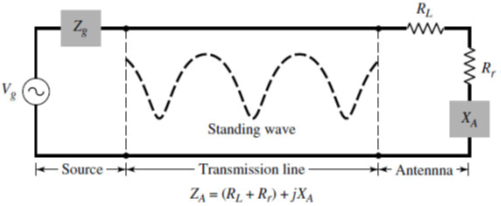
\includegraphics[width=0.8\textwidth]{tline.png}
	\caption{Transmission line Thevenin equivalent of antenna and transmitter}
	\label{fig:tline}
\end{figure} 
To prevent this reflection, the impedances at each end must be matched to the transmission lines characteristic impedance. This can be done through L-section matching, stepped transmission lines or filters.  \\[0.2cm]
L-section is a method used for matching transmission lines; this involves using a capacitor and inductor in a series and parallel combination to match the load. Stepped transmission lines provides impedance matching for lumped elements. Finally, filters can also be used for impedance matching; they are typically used to provide an adjustable match for the circuit over different frequencies. By inserting a filter that is a perfect match for the transmission line at a known frequency \cite{ref9}. This theory will be considered when evaluating the design for the development boards and if required the PCB so they are perfectly matched to reduce any unnecessary losses in the system.

\subsection{Scattering Parameters}
Scattering parameters (S-Parameters) are a matrix that describes the behaviour of linear electrical networks; this matrix is used over a broad range of disciplines of electrical engineering but is particularly useful in microwave engineering.\\
Since the RF switching system this thesis is designing will not generating its own signal or provide any RF front end's; even though the system is switching, it will always have a single input and single output. Therefore, this design can be simplified to be a 2-port network, as shown in Figure \ref{fig:sparam}.
\begin{figure}[H]
	\centering
    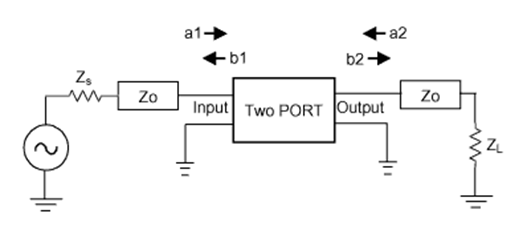
\includegraphics[width=0.8\textwidth]{sparam.png}
	\caption{2-port switching system [10]}
	\label{fig:sparam}
\end{figure} 
2-port networks are most commonly used and can easily be adapted to systems that are more complex, Figure \ref{fig:sparam} shows a simple diagram of a 2-port network and Equation \ref{eq:sparam} shows the matrix and equations given for the network \cite{ref9}.
\begin{align}
\left( \begin{array}{c}
b_1 \\
b_2 \end{array} \right) &=
\left( \begin{array}{cc}
S_{11} & S_{12} \\
S_{11} & S_{12} \end{array} \right)
\left( \begin{array}{c}
a_1 \\
a_2 \end{array} \right) \label{eq:sparam} \\
b_1 &= S_{11}a_1+S_{12}a_2 \nonumber \\
b_2 &= S_{21}a_1+S_{22}a_2 \nonumber
\end{align}
These parameters can be directly measured with a network analyser and will be used to determine the characteristics of the different RF switches.



\subsection{System Losses}
When working with RF and microwave systems it is important to understand the different types of losses that can occur in the system and how it will affect the performance. There are three significant losses to be consider, these are insertion loss, return loss and isolation.\\
Insertion loss is the loss of the signals power in decibels (dB) from the insertion of a device in the input or output of the system. The loss can be determined given the scattering equation of the system, as defined in Equation \ref{eq:ins_loss}.
\begin{align}
Insertion \ loss &= -20\cdot \log_{10}\left( |\Gamma | \right) \label{eq:ins_loss}
\end{align}
The return loss is the loss of the signals power in dB from the signal reflection; this is often caused by an impedance mismatch on the load. The loss can be determined given the reflection coefficient, as shown in Equation \ref{eq:ret_loss}.
\begin{align}
\Gamma &= \frac{Z_L-Z_S}{Z_L+Z_S} \label{eq:ref} \\
Return \ loss &= -20\cdot \log_{10}\left( |\Gamma | \right) \label{eq:ret_loss}
\end{align}
The isolation is the degree of attenuation from other signals from outside or on other channels in the system. Increasing the isolation of the device reduces the influence of other signals. The isolation of the system can be determined by measuring the signal strength at an output where the input is not routed to. \cite{ref9} All of these parameters need to be seriously considered, and form the base of the analysis for the design and development of the RF switching system.

%TODO : Talk about de-embedding systems and embedding systems


\section{RF Switch}
There are two typical types of switches that are used in RF and microwave switching systems, electromechanical switches (EMR) and solid-state switches (SSR). These switches are often available in four different topologies:
\begin{itemize}
	\setlength\itemsep{-0.5em}
	\item Single-pole double-throw (SPDT)
	\item Single-pole-multiple-throw (SPnT)
	\item Double-pole-double-throw (DPDT)
	\item Bypass switch [11]
\end{itemize}
This project is interested in the development of a single input with multiple outputs so will look into utilising combinations of SPDT and SPnT topologies to meet this requirement. \\
Solid-state relay's (SSR) are typically constructed in semiconductor packaging, giving them a small size and are switched by applying an external voltage across its control terminals. Since there are no physical switching mechanisms for SSR, there is no component to wear out allowing the SSR to potentially switch an infinite amount of times. \\
Whereas electromechanical relays (EMR) rely on a mechanical contact to switch the outputs, resulting in an often larger size. Since there is a physical movement required to switch the outputs the EMR, there will be limit on the number of switches before it begins to fail; this is not particularly idea for the RF switching system this thesis is looking at as it will require switches to be replaced after set period depending on its usage. \\
EMR's have a larger frequency range than most SSR's, they support frequencies from DC to the GHz range whereas SSR's often begin around the KHz up to GHz; both switches are ideal as the switch will be working in high frequencies. The insertion loss is often greater in SSR compared to most EMR's but SSR's provide a greater isolation in comparison against EMR. On average, the SSR's provide a greater switching speed with significantly lower settling time making them ideal for high speed switching \cite{ref5}. \\
Both switches have advantages and disadvantages; however, this project looks into the development of a switching system to switch at high speeds with minimal losses, size, noise and power. SSR are the most suitable for meeting these requirements and will therefore be the primary focus of this project.




\section{RF Switches Matrix}
This thesis topic looks into the development of a RF switching system, this will be done by utilising RF and microwave switches to create an RF switching matrix. An RF switch matrix are used to route RF signals from an input to an output.\\
There are several different types of switching matrix's, there is multiple input multiple output (MIMO), multiple input single output (MISO), single input multiple output (SIMO) and single input single output (SISO) \cite{ref12}. For this project we are looking at controlling multiple outputs with a single input, so will be implementing a SIMO RF switching matrix.


\subsection{Switch Architecture}
%Blocking / nonblocking system


\subsection{Switch Topologies}
When constructing a RF switch there are two typical topologies, these are multiplexers and general purpose relays; examples can be seen in Figure 3. General purpose relays are commonly a SPDT or SDnT relay's that are used for routing a signal between multiple paths. Multiplexers are devices that route a single input to multiple outputs or vice versa, they are commonly built from multiple SPDT relays but have a greater inherited insertion loss from this configuration \cite{ref13}.
\begin{figure}[H]
	\centering
    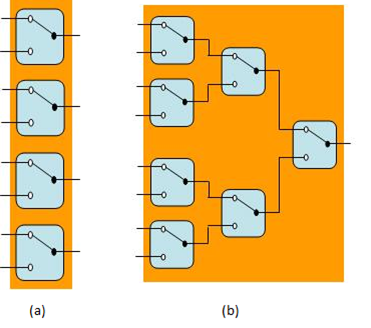
\includegraphics[width=0.8\textwidth]{topology.png}
	\caption{(a) is a Quad SPDT, (b) 8x1 multiplexer}
	\label{fig:topology}
\end{figure} 
Looking at Figure \ref{fig:topology} (b) it can be assumed that there will be losses through each path it takes, insertion loses through first switch, first cable/track, second switch, etc. Therefore, it is ideal to develop a topology as close to Figure \ref{fig:topology} (a) to ensure there is little loss through multiple cascaded switches and cable/tracks. This thesis will be looking into designing a 2x16 MIMO multiplexer, similar to the design in Figure \ref{fig:topology} (b) to provide the available ports as well as a consistent loss through the system.

%TODO : Talk about UFL connectors
\subsection{Cabling}
When developing the RF switching system it is probable to require cables to connect the switches together. If the development boards are used it will be a requirement, and the PCB development could be built into separate daughter boards and connected together via cable. \\
There are three main types of coax cabling:
\begin{itemize}
	\setlength\itemsep{-0.5em}
	\item Semi-rigid
	\item Comfortable
	\item Flexible
\end{itemize}
This project will look into the use of semi-rigid SMA cables, as they typically have low losses for signal transmission and are well suited for fixed devices [16]. The connection between will need to be measured and matched as discussed in Section \ref{sec:tran_theory} to ensure that the signal retains its integrity.




\section{Substrate Selection}
%talk about different available substrates, pros/cons ->how they effect high freq. ->cost
%discuss which are most suitable for this project. MAKE disciosion
There are various substrates that are available for developing the RF switching matrix. Four key substrates were looked at these include:
\begin{itemize} [noitemsep,topsep=0pt]
  \item FR-4
  \item Epoxy
\end{itemize}
Table \ref{tab:substrate} contains the characteristics of these four substrates that are utilised to calculate the dimensions of the RF tracks. 
When designing PCB's for 



%TODO : Replace 'track' with 'transmission line'
\section{RF Transmission Line Design}
%talk about; microstrip, stripline, coplanar. design techniques, 
For designing the RF transmission line on the PCB there are three primary options available
\begin{itemize}[noitemsep,topsep=0.5pt]
	\item Micro-strip
	\item Coplanar Wave-guide, and
	\item Strip-line
\end{itemize}
RF tracks provide ...\\
For designing the tracks we need to consider:
\begin{align}
\lambda&= \frac{c}{f\sqrt{\epsilon_{eff}}} \label{eq:lam} \\
\theta &= \frac{2 \pi}{\lambda} \label{eq:phase}
\end{align}
We need to consider the Figure \ref{eq:lam} and \ref{eq:phase} as these are the fundamentals for designing any type of track. To determine which track is best suited this thesis will look at each available option.\newline
%------
These equations are used for the approximate design of RF tracks, in order to obtain a more precise design which consider a wider range of variables dedicated software is  used to further verify the design of the tracks.
%REFERENCE

\subsection{Micro-strip}
Microstrip RF tracks are the most common RF transmission line currently used in practice. %NEED TO CITE THIS!!!!
%---------------------
% need to talk about microstrip in general
%----------------------
\fig{fig:microdiag} presents a typical microstrip which has been labelled the critical dimensions of this transmission line. \newline
\begin{figure}[H]
	\centering
    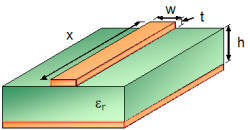
\includegraphics[width=0.65\textwidth]{microdiag.jpg}
	\caption{Microstrip diagram}
	\label{fig:microdiag}
\end{figure} 
We are able to calculate the dimensions shown in \fig{fig:microdiag} by using the following:
\begin{align}
W&=\frac{t}{\pi} \left[ ln \left( \frac{2h}{t} \right) +1 \right] \\
H&=h-2t 
\end{align}
\begin{numcases}{\epsilon_{eff}=}
	\frac{\epsilon_r+1}{2} + \frac{\epsilon-1}{2} \left[ \frac{1}{\sqrt{1+\frac{12H}{W}}} +0.04 \left(1- \frac{W}{H} \right)^2 \right] &$when \left( \frac{W}{H} \right) < 1$  \label{eq:epsh<1} \\
	\frac{\epsilon+1}{2}+ \frac{\epsilon-1}{2\sqrt{1+\frac{12H}{W}}} & $when \left( \frac{W}{H} \right) > 1$  \label{eq:epsh>1}
\end{numcases}
\begin{numcases}{Z_0=}
   \frac{60}{\sqrt{\epsilon_{eff}}} \cdot ln\left( \frac{8H}{W}+\frac{W}{4H} \right), & $when \left( \frac{W}{H} \right) < 1$  \label{eq:microh<1} \\
   \frac{120 \pi}{\sqrt{\epsilon_{eff}} \cdot \left[ \frac{W}{H}+1.393+\frac{2}{3}ln \left(\frac{W}{H}+1.444 \right) \right]}, & $when \left( \frac{W}{H} \right) > 1$ \label{eq:microh>1}
\end{numcases}
In order to calculate the dimensions of the micro-strip track we are required to make key decisions for the design. By selecting the frequency range, impedance, phase shift substrate and track thickness we are able to determine the dimensions for the track. \newline
We are able to determine the width ($W$) and length($X$) of the track by selecting a substrate determining the dielectric constant ($\epsilon_{eff}$), copper thickness ($t$) and height($H$). We can set the 


%why we should use this, characteristics, limitations ect.


\subsection{Strip-line}
Strip-line RF tracks are ... \newline

We are able to calculate the dimensions shown in Figure 3.2


\begin{align}
\beta&=\frac{\omega}{v_p} 	\nonumber \\
&= \sqrt{\epsilon_r} \cdot k_0	\label{eq:stripline:beta}\\
Z_0&= \sqrt{\frac{L}{C}} \nonumber \\
	&=\frac{1}{v_p \cdot C}	\label{eq:stripline:impedance}
\end{align}


\begin{numcases}{\frac{W_e}{b}=}
	\frac{W}{b} & $when \left( \frac{W}{b} \right) > 0.35$  \label{eq:stripline:wb>0.35} \\
	\frac{W}{b}-\left(0.35-\frac{W}{b} \right)^2 & $when \left( \frac{W}{b} \right) < 0.35$  \label{eq:stripline:wb<0.35}
\end{numcases}

\begin{numcases}{\frac{W}{b}=}
	x &$when \sqrt{\epsilon_r} \cdot Z_0<120\ohm$  \label{eq:stripline:<120} \\
	0.85 - \sqrt{0.6-x} & $when \sqrt{\epsilon_r} \cdot Z_0<120\ohm$  \label{eq:stripline:>120}
\end{numcases}

\begin{align}
x=\frac{20 \pi}{\sqrt{\epsilon_r \cdot Z_0}}	\label{eq:stripline:x}
\end{align}

\subsection{Coplanar Wave-guide}
C












%Physical Enclosure & track losses
\section{Radiation Emission}


\subsection{Picket Fencing Technique}	\label{sec:picket}


\subsection{Shielding}


%---------------------------------------------------------------------------------








%---------------------------------------------------------------------------------
%Possibly remove this section of the report
\chapter{RF Switch Evaluation}
In this chapter the design of discrete RF switches is evaluated in comparaison to commercially available switches. This chapter will look into the design and simulations of SPDT, SP4T and SP8T RF switches within the frequency range of 100MHz-4GHz to gain a better understanding of RF switch functionality and variants.
 
\section{RF Switch Design}
There are two 


\subsection{PIN Diode}


\subsection{FET}

\section{Topologies}



\section{Available RF Switches}

%---------------------------------------------------------------------------------
 






%---------------------------------------------------------------------------------
\chapter{Methodology}
This chapter of the thesis looks at the methodology employed in the design and development of the RF switch matrix. For this Thesis the design stage has been broken into five primary sections:\\[-0.8cm]
\begin{itemize}
	\setlength\itemsep{-0.5em}
	\item Evaluation of RF switches
	\item Design a switch matrix
	\item Develop PCB design
	\item Evaluate the RF switch matrix
	\item Construction of matrix enclosure
\end{itemize}
These sections will be further discussed to analyse the progression of the design and development of the RF switch matrix.

\section{Evaluation}
This section looks at evaluating the currently available RF switch evaluation boards listed in Section \ref{sec:evalboard_eval} that can be used, and alternative possibilities in developing a custom RF switch matrix.

\subsection{Evaluation Boards}		\label{sec:evalboard_eval}
We currently have $4$ evaluation RF switch boards available; these include:
\vspace{-0.5em}
\begin{table}[H]
	\centering
	\begin{tabular}{p{5cm} r}
	asdf & $\$50$ USD \\
	asdf & $\$50$ USD\\
	asdf & $\$50$ USD\\	
	\end{tabular}
\end{table} 
\vspace{-4mm}
The three available evaluation boards we investigated using a \model \ Vector Network Analyser (VNA); each switch was wired so that the input is connected to the output, while all other ports were $50\ohm$ terminated. The switch was powered and the controls set to allow the signal to propagate down the open path, then changed the state to have a closed path; this was conducted for each evaluation board. The results were exported to a \textit{.s2p} file to be analysed using ADS, and the results can be seen in Appendix \ref{sec:eval_res} 's Figure's \ref{fig:res:}, \ref{fig:res:} \& \ref{fig:res:}. \\
These simulations \\
The results of ... 
%the good board
is the most ideal RF switch out of the three boards, but the overall price to construct the switch matrix is far too expensive to construct as it will cost $\$50$ which is unrealistic to rival 


\subsection{RF Switches}
It was seen in previous section that the EMR and 
%TODO : Is it a switch matrix
switch relay provided significantly better results for: insertion, isolation and reflection but are significantly larger and heavier than SSR's tested. Since this thesis is looking at developing a lightweight switch matrix it is decided that high performance SSR's will be looked at instead of EMR. \\[0.2cm]
For constructing the switch matrix there are three primary topolgies that will be looked at since, SP16T are not largely available at a low price, instead this thesis will look at cascading two or more switches that are SPDT, SP4T or SP8T; to create a custom SP16T switch.\\
There is a large variety of RF switches available in varying topologies, the following RF switches were identified as interesting:\\[-0.8cm]
\begin{table}[H]
	\centering
	\begin{tabular}{p{5cm} r}
	asdf & $\$50$ USD \\
	asdf & $\$50$ USD\\
	asdf & $\$50$ USD\\	
	\end{tabular}
\end{table} 
\vspace{-4mm}
These are the RF switches that will be further investigated in this thesis to determine if a custom RF switch design is able to constructed at a competitive price to the evaluation boards seen in Section \ref{sec:evalboard_eval}. It can already be seen that the individual price is significantly cheaper but will require a PCB to be constructed; this will allow the design to be custom designed to fit in the most space efficient package possible to allow for a portable and lightweight design. 

\subsection{Transmission Line Design}
Using the ADS three different transmission lines were tested, using the parameters seen in Appendix \ref{sec:substrate_param}, Table \ref{tab:tracks} was constructed.\begin{table}[H]
	\centering
	\begin{tabular}{L{4cm} C{3cm} C{3cm} C{3cm}}
		\hline
		Track Type & Width & Length & Gap \\
		\hline
		Micro-strip & & & -\\
		Strip-line & & & -\\
		Co-planar Wave-guide & & &\\
		\hline
	\end{tabular}
	\caption{Transmission Line Design Parameters}
	\label{tab:tracks}
\end{table} 
\vspace{-2mm}
Therefore looking at Table \ref{tab:tracks} it can be seen that the most space efficient transmission line is the CPWG design; therefore, the CPWG design allows the PCB to be the most space efficient design for the RF switch design.\\
In addition to the Grounded CPWG, picket fencing will be added to the tracks to ensure that there is minimal amount of losses or noise entering the system as seen in Section \ref{sec:picket}.
%TODO : talk about picket fencing




\section{Design}
For the design of the RF switch matrix, several key design citerias were identified to be required for the final product of the switch matrix; these specifications are:
\begin{itemize}
	\setlength\itemsep{-0.5em}
	\item Two RF inputs
	\item Sixteen RF outputs
	\item Maximum path loss of $3$dB
	\item Power-able from low-power device (such as USB)
	\item Input and output of switch matrix are $50\ohm$
\end{itemize}
%TODO : talk about the general design
%TODO : mention that the design is blocking, two signals cant add together on the output.
In order to construct the DP16T switch matrix the the design will be split into two stages, an input and output stage. The input stage will take a two different inputs, the switch will be controlled to route a path from the input to the output; this will require two separate SP16T RF switch. Each output of DP16T matrix needs to be able to switch between the two outputs of each SP16T switch, therefore this design will require 16 SPDT switches. \\[0.2cm]
In order to meet these specifications several different designs have been developed, which can be seen in Section \ref{sec:design1} - \ref{sec:output2}. There are three different SP16T switch designs for the input and two SPDT output switch designs for the output; to determine the most suitable design these five designs are designed to determine a suitable low-loss, high isolation switch matrix. \\[0.2cm]
All the design's for the SP16T switches will feature an SMA input for the input to the switch matrix, and UFL connectors on the output. Since the internals of the design will be restricted from the consumer UFL cabling allows for a much more compact and flexible design. This selection is expected to have a poor insertion loss compared to SMA but is significantly more flexible and thinner allowing for the overall size of the switch matrix to be reduced significantly.\\
The output switches will feature a similar design; where the input to the SPDT switch is SMA and the two outputs will be UFL. The SPDT switch will need to be $50\ohm$ terminated when inactive to ensure that there isn't any reflections occurring within the switch if the signal is being routed to the same output, since the design in a blocking switch matrix.  

\subsection{Design 1}		\label{sec:design1}
This design looks at constructing a SP16T RF switch using the SKY13418-485LF and MASWSS0115 cascaded together. The SKY13418 is a SP8T switch that provides a low insertion loss that has a frequency range from $100$MHz to $3$Ghz.  The chip features the input in the centre with $4$ outputs either side of the input. This allows for the tracks to be spaced by $30^o$ segments, and the remainder to be space for logic. To get full 16 outputs the design requires a MASWSS0115 SPDT switch on each output of the SP8T; from the switches that are being evaluated the MASWSS0115 provides the lowest insertion loss, although it has a poor reflection on the output. The SKY13418 has DC blocking integrated into the chip by the MASWSS0115 doesn't, therefore it requires DC blocking capacitors of $33$\pF \ to be placed on all of the RF inputs and outputs. \\[0.2cm]
This design was developed in Altium Designer and can be seen in Figure \ref{fig:design1}.
\begin{figure}[H]
	\centering
    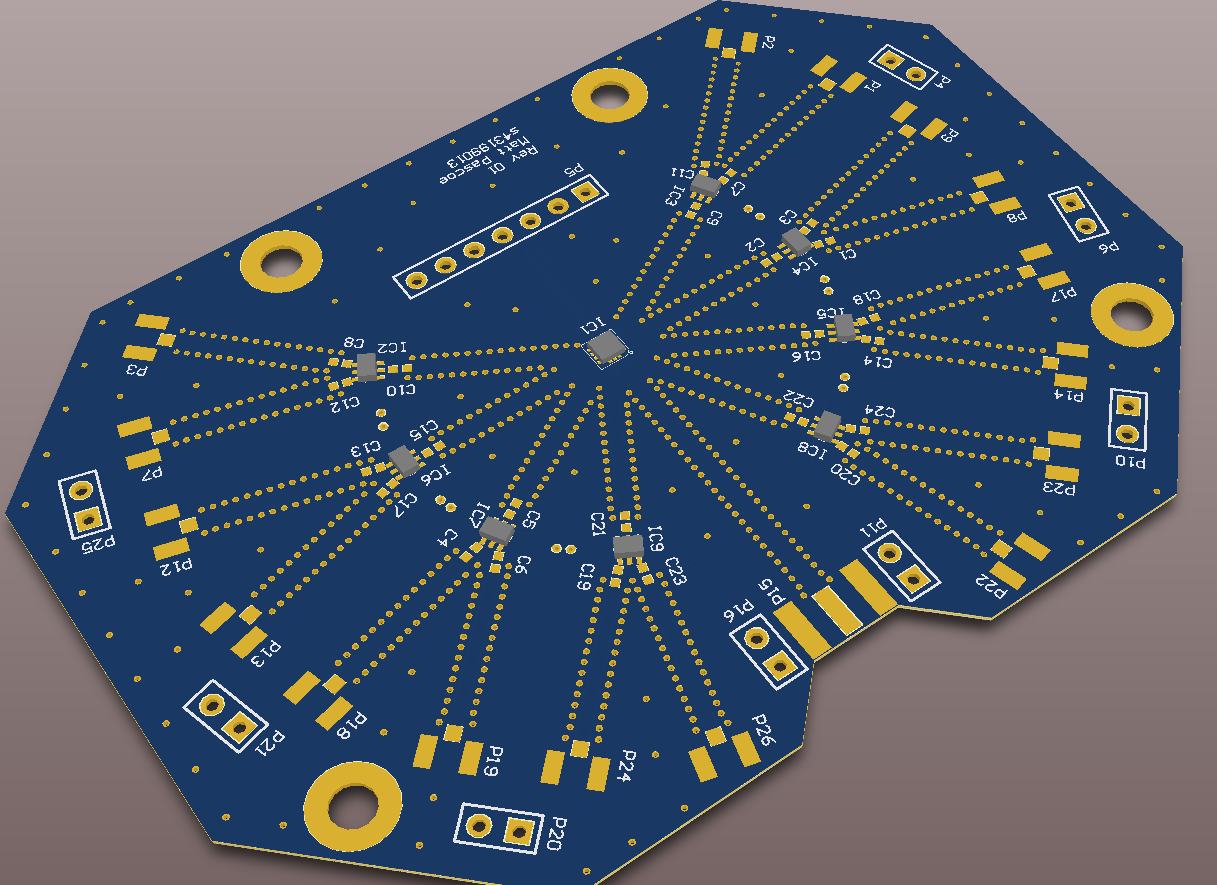
\includegraphics[width=0.8\textwidth]{design1_pcb.png}
	\caption{PCB Design for `Design 1'}
	\label{fig:design1}
\end{figure} 
\subsubsection{Specifications}
Therefore using this combination of SP8T and SPDT switches we are able to estimate the parameters of the switch based off of the specifications in the data-sheet as seen in Table \ref{tab:des1_param}.
\begin{table}[H]
	\centering
	\begin{tabular}{| L{4cm} | C{1.5cm} | C{1.5cm} | C{1.5cm} | C{1.5cm} | C{1.5cm} |}
		\hline
		\multicolumn{1}{|c|}{\multirow{2}{*}{Parameter}} & \multicolumn{5}{c|}{Value}\\
		\cline{2-6}
		& $100$MHz & $1$GHz & $2$GHz & $3$GHz & $4$Ghz \\
		\hline
		Insertion & & & & &\\
		\noalign{\hrule height 0.01pt}
		Isolation & & & & & \\
		\noalign{\hrule height 0.01pt}
		Input Reflection & & & & & \\
		\noalign{\hrule height 0.01pt}
		Output Reflection (Inactive) & & & & & \\
		\noalign{\hrule height 0.01pt}
		Max. Switching Speed & & & & &\\
		\hline
	\end{tabular}
	\caption{Design 1 - Ideal parameters}
	\label{tab:des1_param}
\end{table}
It can be seen that the expected insertion loss is relatively low at a maximum of $1$dB loss, the isolation is not too bad with a minimum of $1$dB. 
%TODO : discuss why this is a good design based on table results
%TODO : talk about the frequency range of the switch
%TODO : talk about the maximum input power
%TODO : 

\subsubsection{Control}
In order to control this  board there are $3$ control pins for the SP8T switch, and $16$ control pins for the SPDT switches. The logic voltages for this board are detailed in Table \ref{tab:design1_logic_v}.
\begin{table}[H]
	\centering
	\begin{tabular}{L{3cm}C{3cm}C{3cm}}
	\hline
	RF Switch & On & Off\\
	\hline
	SP8T & $0$V$\pm 0.3V$ & $1.35$V - $2.7$V \\
	SPDT & $0$V$\pm 0.2V$ & $2.3$V - $5$V\\
	\hline	
	\end{tabular}
	\caption{Logic Voltage Control}
	\label{tab:design1_logic_v}
\end{table}
Therefore this the device can be controlled using a $4$-bit number representing the current active switch for the input. A logic table has been drawn to design a suitable method to control the SP16T switch with minimal amount of cabling and components required; the results can be seen in Appendix \ref{sec:logic_design1}. Therefore this design can be easily controlled using the output logic from the micro-controller where the output signal is $4$-bits, the first bits are connected to each SPDT switch and the last three bits are connected to the SP8T switch.

\subsection{Design 2}		\label{sec:design2}
This design looks at constructing an alternative design to SP16T RF switch using a different topology from Section \ref{sec:design1}; it was found that the SP4T PE42441 Evaluation Board tested in Section \ref{sec:evalboard_eval} provided good performance for both insertion and isolation. By cascading the SP4T together with itself would provide $16$ possible transmission lines for the switch. By using the same transmission line design used in Design 1, an alternative construction of the SP16T switch can be designed. By designing this board on a PCB it is able to significantly more space efficient, cost effective with less cabling than what would be required to construct it from the tested evaluation board seen in Section \ref{sec:evalboard_eval}.\\[0.2cm]
The pins on the PE42441 were spaced so that the transmission lines could be angled $45^o$ apart from each other. This was done for each chip leading from the SMA to UFL. Similar to `Design 1' the track length was designed to provide enough spacing for the PE42441 chips and UFL connectors from each other and the header connectors. The chips do not require DC blocking so no capacitors are required on the input or outputs; following the specifications on the PE42441's data-sheet, 0.1\uF decoupling capacitors were added to the $V_{cc}$, $V_0$ and $V_1$. 
\\[0.2cm]
This design was developed in Altium Designer and can be seen in Figure \ref{fig:design2}.
\begin{figure}[H]
	\centering
    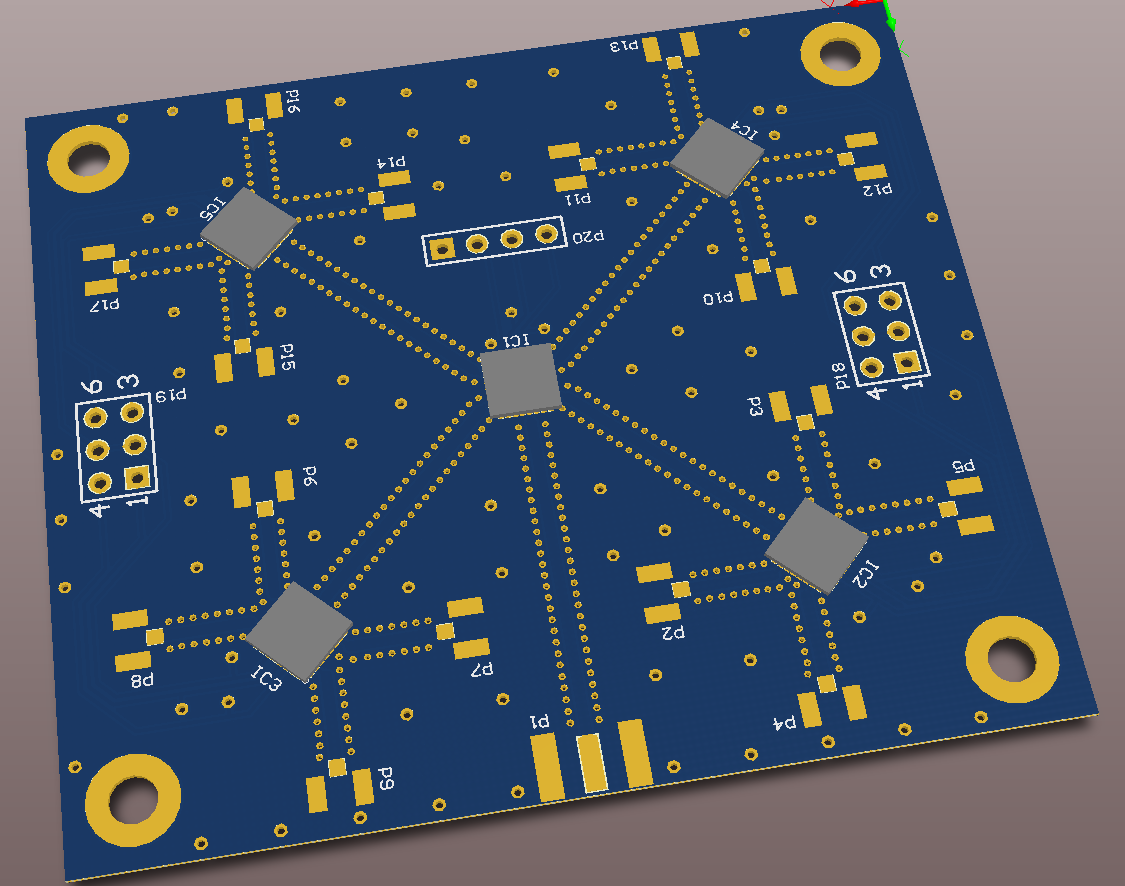
\includegraphics[width=0.8\textwidth]{design2_pcb.png}
	\caption{PCB Design for `Design 2'}
	\label{fig:design2}
\end{figure} 

\subsubsection{Specifications}
Therefore using the SP4T switches cascaded together the performance of the switch can be estimate the parameters of the switch based off of the specifications presented in the PE42441's data-sheet; the estimated performance can be seen in Table \ref{tab:des1_param}.
\begin{table}[H]
	\centering
	\begin{tabular}{| L{4cm} | C{1.5cm} | C{1.5cm} | C{1.5cm} | C{1.5cm} | C{1.5cm} |}
		\hline
		\multicolumn{1}{|c|}{\multirow{2}{*}{Parameter}} & \multicolumn{5}{c|}{Value}\\
		\cline{2-6}
		& $100$MHz & $1$GHz & $2$GHz & $3$GHz & $4$Ghz \\
		\hline
		Insertion & & & & &\\
		Isolation & & & & & \\
		Input Reflection & & & & & \\
		Output Reflection & & & & & \\
		Max. Switching Speed & & & & &\\
		\hline
	\end{tabular}
	\caption{Design 1 - Ideal parameters}
	\label{tab:des1_param}
\end{table}
It can be seen that the expected insertion loss is relatively low at a maximum of $1$dB loss, the isolation is not too bad with a minimum of $1$dB. 
%TODO : discuss why this is a good design based on table results
%TODO : talk about the frequency range of the switch
%TODO : talk about the maximum input power
%TODO : 

\subsubsection{Control}
In order to control this  board there are $3$ control pins for the SP8T switch, and $16$ control pins for the SPDT switches. The logic voltages for this board are detailed in Table \ref{tab:design2_logic_v}
\begin{table}[H]
	\centering
	\begin{tabular}{L{3cm}C{3cm}C{3cm}}
	\hline
	RF Switch & On & Off\\
	\hline
	SP4T & $0$V$\pm 0.3V$ & $1.35$V - $2.7$V \\
	\hline	
	\end{tabular}
	\caption{Logic Voltage Control}
	\label{tab:design2_logic_v}
\end{table}
Therefore this the device can be controlled using a $4$-bit number representing the current active switch for the input. A logic table has been drawn to design a suitable method to control the SP16T switch with minimal amount of cabling and components required; the results can be seen in Appendix \ref{sec:logic_design1}. Therefore this design can be easily controlled using the output logic from the micro-controller where the output signal is $4$-bits, the first two bits are connected to each of the cascaded SP4T switches and the last two bits are connected to the centre SP4T switch.


\subsection{Design 3}		\label{sec:design3}
This design looks at constructing a SP16T RF switch using an similar design to Design 2, this utilises the PE42442 chip which is from the same family as the PE42441. Similar to teh PE42441, the PE42442 is a SP4T RF switch that slightly varries in their specifications. The PE42442 provides a lower input power, but provides a slightly better insertion and isolation response than the PE42441.\\[0.2cm]

The device is able to be compacted into a smaller board due to the alternate arrangement of pins in comparison to Design 2; this new Altium design can be seen in Figure \ref{fig:design3}.

This design was developed in Altium Designer and can be seen in Figure \ref{fig:design3}.
\begin{figure}[H]
	\centering
    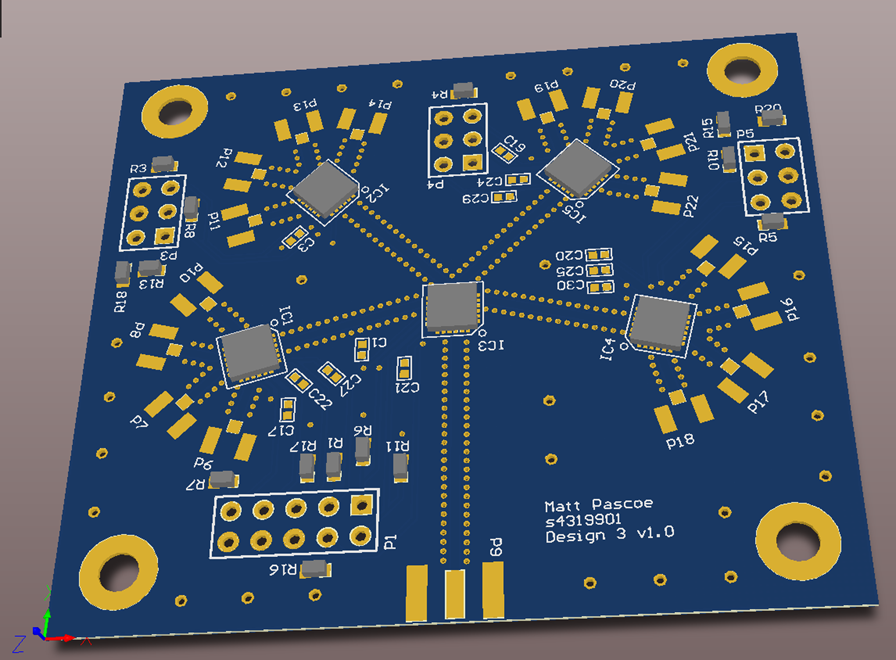
\includegraphics[width=0.8\textwidth]{design3_pcb.png}
	\caption{PCB Design for `Design 3'}
	\label{fig:design3}
\end{figure} 

\subsubsection{Specifications}
Therefore using the SP4T switches cascaded together the performance of the switch can be estimate the parameters of the switch based off of the specifications presented in the PE42442's data-sheet; the estimated performance can be seen in Table \ref{tab:des1_param}.
\begin{table}[H]
	\centering
	\begin{tabular}{| L{4cm} | C{1.5cm} | C{1.5cm} | C{1.5cm} | C{1.5cm} | C{1.5cm} |}
		\hline
		\multicolumn{1}{|c|}{\multirow{2}{*}{Parameter}} & \multicolumn{5}{c|}{Value}\\
		\cline{2-6}
		& $100$MHz & $1$GHz & $2$GHz & $3$GHz & $4$Ghz \\
		\hline
		Insertion & & & & &\\
		Isolation & & & & & \\
		Input Reflection & & & & & \\
		Output Reflection & & & & & \\
		Max. Switching Speed & & & & &\\
		\hline
	\end{tabular}
	\caption{Design 1 - Ideal parameters}
	\label{tab:des1_param}
\end{table}
It can be seen that the expected insertion loss is relatively low at a maximum of $1$dB loss, the isolation is not too bad with a minimum of $1$dB. 
%TODO : discuss why this is a good design based on table results
%TODO : talk about the frequency range of the switch
%TODO : talk about the maximum input power
%TODO : 

\subsubsection{Control}
In order to control this  board there are $3$ control pins for the SP8T switch, and $16$ control pins for the SPDT switches. The logic voltages for this board are detailed in Table



\subsection{Output 1}		\label{sec:output1}
The output design requires constructing a SPDT switch for the output of the RF switch matrix, this requires a switch that has low insertion loss and isn't reflective. The switch should also include 


This design was developed in Altium Designer and can be seen in Figure \ref{fig:output1}.
\begin{figure}[H]
	\centering
    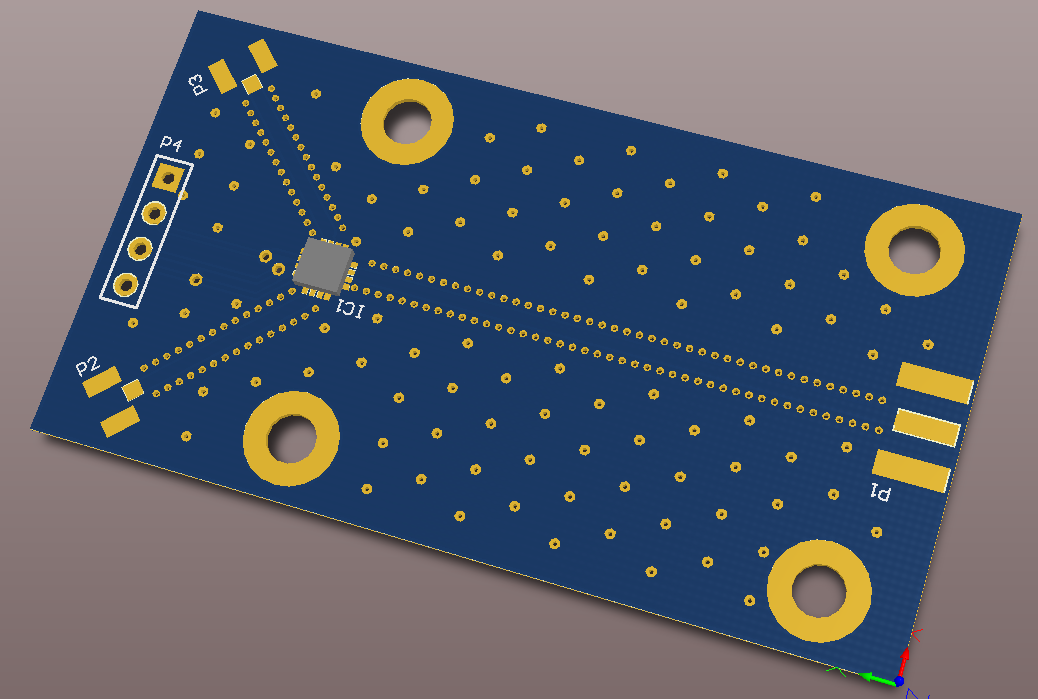
\includegraphics[width=0.8\textwidth]{output1_pcb.png}
	\caption{PCB Design for `Output 1'}
	\label{fig:output1}
\end{figure} 

\begin{table}[H]
	\centering
	\begin{tabular}{| L{4cm} | C{2cm} | C{2cm} | C{2cm} | C{2cm} |}
		\hline
		\multicolumn{1}{|c|}{\multirow{2}{*}{Parameter}} & \multicolumn{4}{c|}{Value}\\
		\cline{2-5}
		& $1$GHz & $2$GHz & $3$GHz & $4$Ghz \\
		\hline
		Insertion & & & & \\
		Isolation & & & & \\
		Input Reflection & & & & \\
		Output Reflection & & & & \\
		Max Switching Speed & & & &\\
		\hline
	\end{tabular}
	\caption{Design 3 Ideal parameters}
	\label{tab:des3_param}
\end{table}
%TODO : discuss why this is a good design based on table results


\subsection{Output 2}		\label{sec:output2}
%TODO : show pcb board
This design looks at constructing a SP16T RF switch using 
\begin{table}[H]
	\centering
	\begin{tabular}{| L{4cm} | C{2cm} | C{2cm} | C{2cm} | C{2cm} |}
		\hline
		\multicolumn{1}{|c|}{\multirow{2}{*}{Parameter}} & \multicolumn{4}{c|}{Value}\\
		\cline{2-5}
		& $1$GHz & $2$GHz & $3$GHz & $4$Ghz \\
		\hline
		Insertion & & & & \\
		Isolation & & & & \\
		Input Reflection & & & & \\
		Output Reflection & & & & \\
		Max Switching Speed & & & &\\
		\hline
	\end{tabular}
	\caption{Design 3 Ideal parameters}
	\label{tab:des3_param}
\end{table}
%TODO : discuss why this is a good design based on table results


\section{Development}
This section looks at the development of the RF switch matrix.



\subsection{PCB Development}

%TODO : talk about the pcb design stage, ads calculations and simulations
One of the key design parameters is for developing a portable device, this requires the switch matrix to be as small as possible. To determine the best solution ADS's LineCalc is used to % 


%TODO : talk about the altium design, physical requirements/limitations


\subsection{RF Switch Development}
After the design of the PCB had been completed the order was processed by a PCB development company. During this project two companies were used: PCBZone and PCBWay. The key difference between these companies was price, quantity and quality; 

%TODO : Breif discsusion about the soldering and selection of chips and capacitors
The RF switch chips that were selected are only available in QFN, .... or ... packages; this limited the design capabilities to SMD




\section{Physical Construction}
%TODO : talk about PCB development/soldering/stands/mounts/cabling


%TODO : talk about the case development/sizing/mounting






%TODO : device selection
\section{Micro-controller Development}		\label{sec:micro_dev}
In order to control and operate the RF Switch system a some type of micro-controller is required to be used to switch the inputs and outputs of the system. The micro-controller needs to meet the following key design parameters:
\begin{itemize}
	\setlength\itemsep{-0.5em}
	\item Capable of supporting .... control pins.
	\item Enable a switch speed of $100$\ns
	\item Low power requirements, less than $5$\W
	\item Source power from USB, and communicate using $15260$ Baud rate.
	\item Capability to sync other controllers, 
\end{itemize}
The ideal device is a low-powered micro-controller, for this project the PSOC4-BLE has been selected to ensure that it is able to control the 


%TODO : Flow chart, block diagram
\subsection{Design}



For each development board a logic table was developed, the table for the .... can be seen in Table \ref{tab:logic_design}. This table determines the logic required to ensure that the control is kept to its most simplistic form.
\begin{table}
	\centering
	%insert table from appendicies
	\caption{Design ... Logic Table}
	\label{tab:logic_design}
\end{table}
Therefore using this we are able to determine:

\subsection{Evaluation}


%---------------------------------------------------------------------------------









%---------------------------------------------------------------------------------
\chapter{Verification}

\section{Individual Board's}	\label{sec:indv_boards}
This section looks at the results obtain from each of the individual boards, each board was tested with a \model \ VNA. By evaluating these boards it can be determined which is most suited for the final design of the RF switch matrix; Section \ref{sec:res_des1} - \ref{sec:res_out2} details the analysed results and discuses the benefits and disadvantages of that design. 


\subsection{Design 1}	\label{sec:res_des1}
The design for `Design 1' which was designed in Section \ref{sec:design1} was constructed and developed according to the design. This section looks at analysing the SP16T RF switch developed to determine the losses, speed and power requirements of the design and comparing them against the specifications detailed in the RF switches data-sheet.\\
A \model \ VNA is used to analyse the SP16T; this is used to determine the losses of the system, the micro-controller is used to increment the switch speed of the device to determine the frequency where the SP16T is unable to maintain the losses seen in the previous section. Finally the 
 
\subsubsection{Losses}
Design 1 has been tested with a VNA to obtain $3$ different results for the device which shows an open transmission line seen in Figure \ref{fig:design1_1}. Additional tests were conducted to determine the effects of the SP16T when one or all of the switches are closed to determine the internal reflections of the device; these results can be seen in Figure \ref{fig:design1_2} - \ref{fig:design1_3}.

\begin{figure}[H]
	\centering
	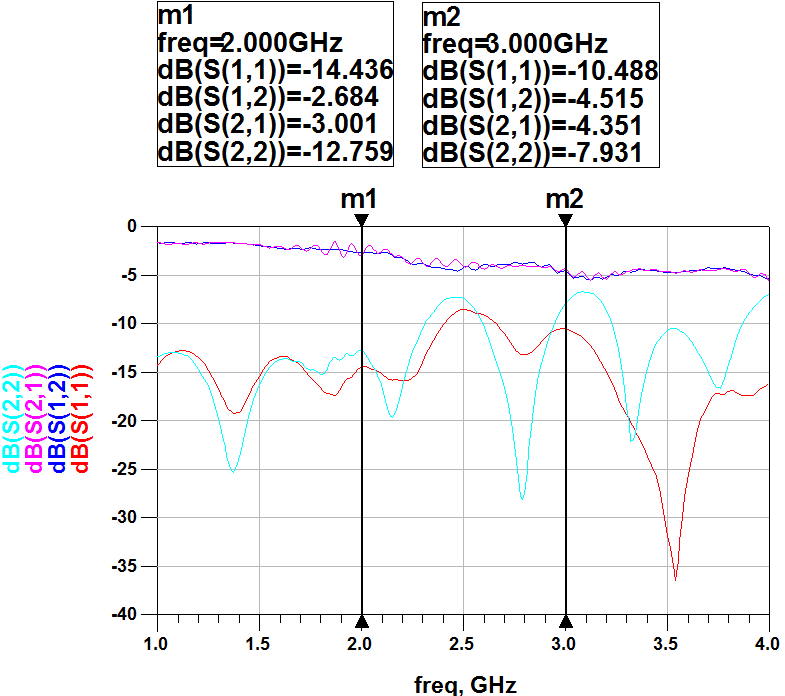
\includegraphics[width=0.75\textwidth]{Design1-1.png}
	\caption{Design 1 S-Parameters - Insertion Loss}
	\label{fig:design1_1}
\end{figure} 
\begin{figure}[H]
	\centering
	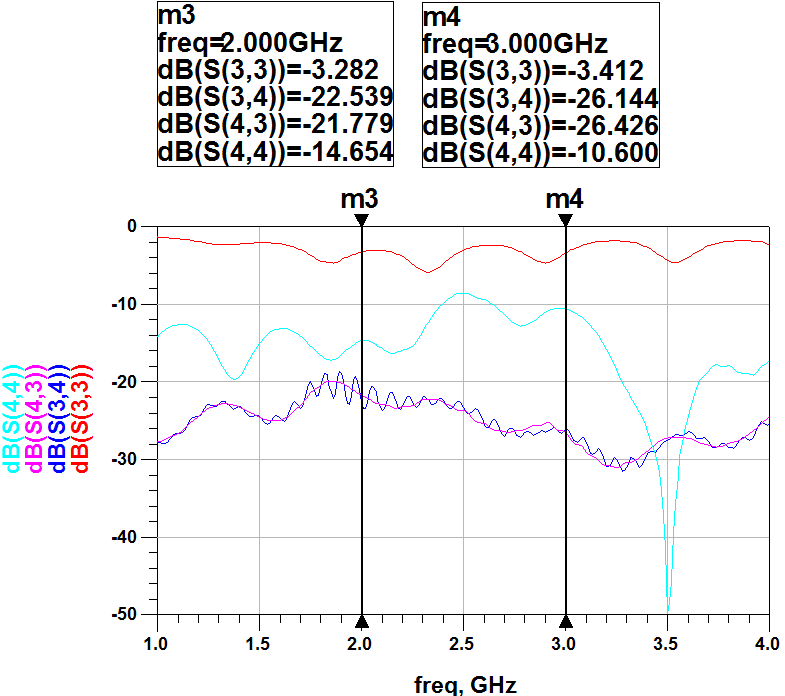
\includegraphics[width=0.75\textwidth]{Design1-2.png}
	\caption{Design 1 S-Parameters - Isolation (Best case)}
	\label{fig:design1_2}
\end{figure} 
\begin{figure}[H]
	\centering
	%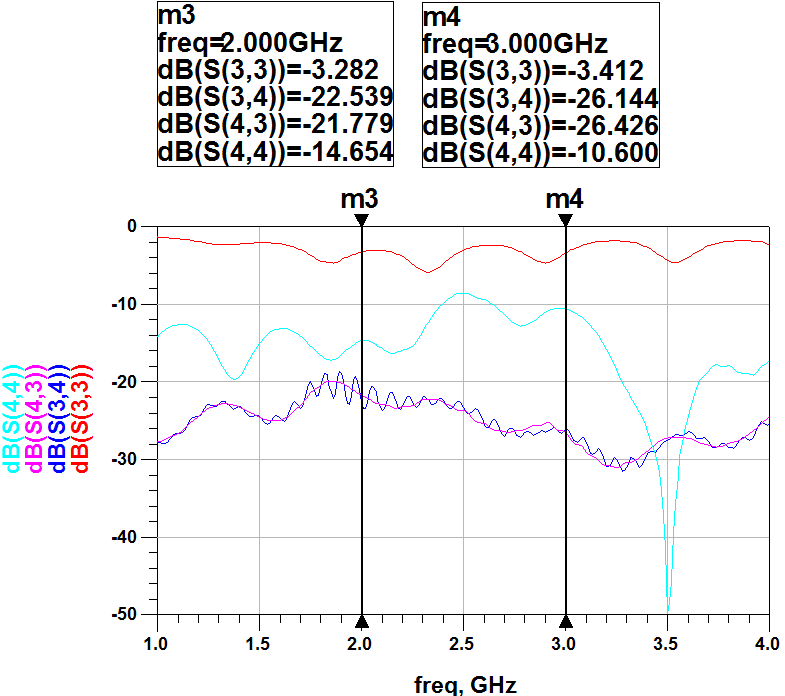
\includegraphics[width=0.75\textwidth]{Design1-2.png}
	\caption{Design 1 S-Parameters - Isolation (Worst case)}
	\label{fig:design1_3}
\end{figure} 

It can be seen looking at the results that the results obtained in Figure \ref{fig:design1_sma}
%Talk about the following results
%TODO : S11 input reflection

%TODO : S12 input insertion

%TODO : S21 output insertion

%TODO : S22 output reflection

\subsubsection{Power Requirements}









\subsection{Design 2}
The design for `Design 2' which was completed in Section \ref{sec:design2} was constructed and developed according to the design. This section looks at analysing the SP16T RF switch developed to determine the losses, operation requirements of this design against the specifications detailed in the RF switches data-sheets. \\[0.2cm]
It was found that this board was not functioning, after wiring the board upto the micro-controller it was found that the changing the logic on the centre PE42441 chip didn't make a significant change to the insertion of the board. Whereas changing the logic on the second PE42441 chip cascaded had a small change on the insertion loss of the device; this change can be seen in Figure \ref{fig:design2_1} and \ref{fig:design2_2}.
\begin{figure}[H]
	\centering
	%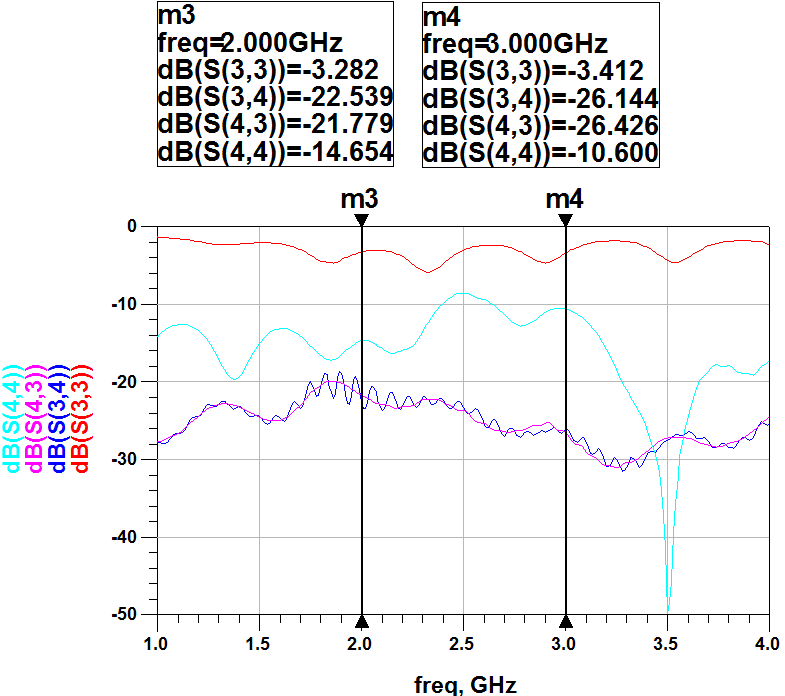
\includegraphics[width=0.75\textwidth]{Design1-2.png}
	\caption{Design 2 S-Parameters - Insertion (Best case)}
	\label{fig:design2_1}
\end{figure} 
\begin{figure}[H]
	\centering
	%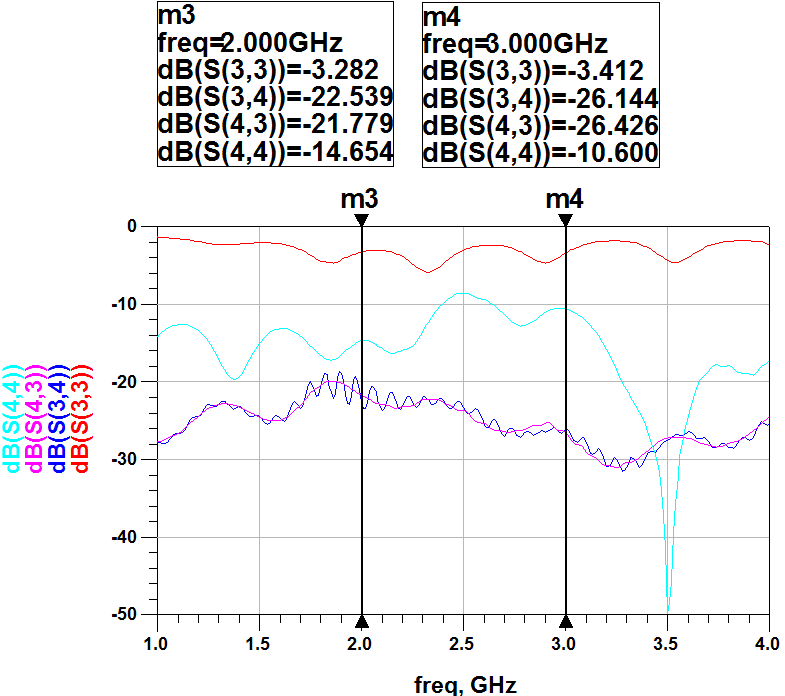
\includegraphics[width=0.75\textwidth]{Design1-2.png}
	\caption{Design 2 S-Parameters - Insertion (Worst case)}
	\label{fig:design2_2}
\end{figure} 
Therefore it can be seen that there is an issue within the first chip, this issue is likely due to an issue from soldering. 

Therefore, due to time constraints of the thesis this design was terminated as the design expectations from Section \ref{sec:design2} had poorer insertion losses than the `Design 1' or `Design 3' so under the allocated budget was not worth further investigating.   







\subsection{Design 3}
The design for `Design 3' which was designed in Section \ref{sec:design3} was constructed and developed according to the design. This section looks at analysing the SP16T RF switch developed to determine the losses, speed and power requirements of the design and comparing them against the specifications detailed in the RF switches data-sheet.\\
A \model \ VNA is used to analyse the SP16T; this is used to determine the losses of the system, the micro-controller is used to increment the switch speed of the device to determine the frequency where the SP16T is unable to maintain the losses seen in the previous section. Finally the 
 
\subsubsection{Losses}
Design 3 has been tested with a VNA to obtain $3$ different results for the device which shows an open transmission line seen in Figure \ref{fig:design3_1}. Additional tests were conducted to determine the effects of the SP16T when one or all of the switches are closed to determine the internal reflections of the device; these results can be seen in Figure \ref{fig:design3_2} - \ref{fig:design3_3}. 

\begin{figure}[H]
	\centering
	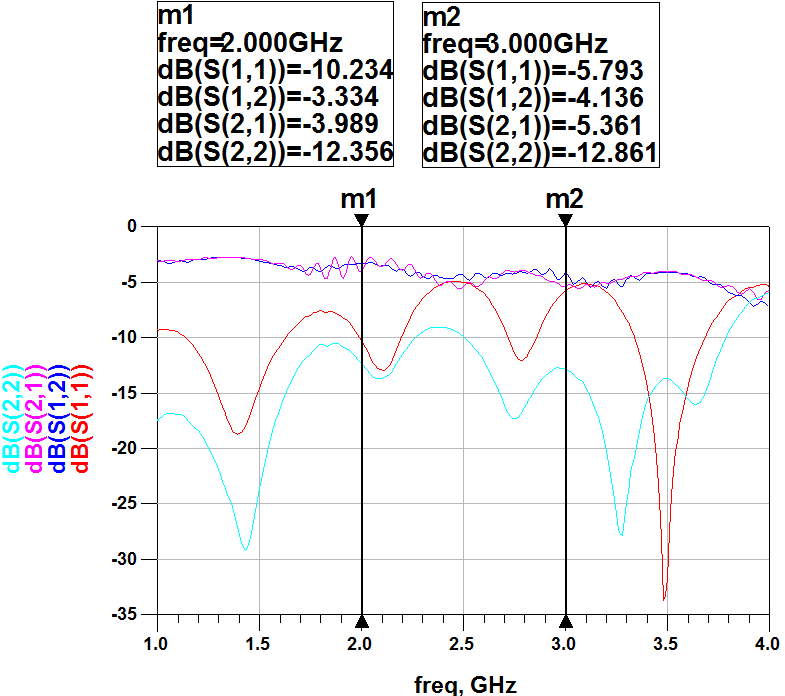
\includegraphics[width=0.75\textwidth]{Design3-1.png}
	\caption{Design 1 S-Parameters - Insertion Loss}
	\label{fig:design3_1}
\end{figure} 
\begin{figure}[H]
	\centering
	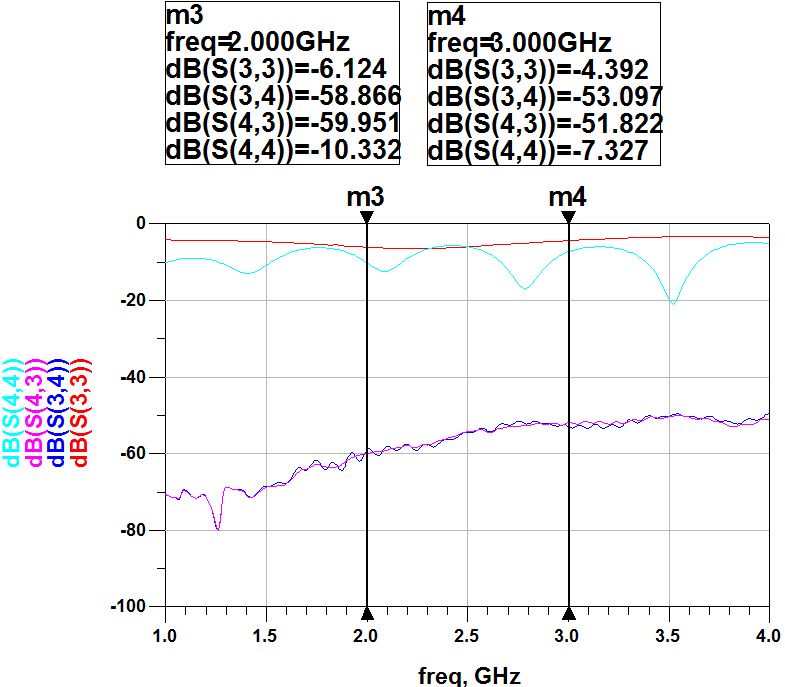
\includegraphics[width=0.75\textwidth]{Design3-2.png}
	\caption{Design 1 S-Parameters - Isolation (Best case)}
	\label{fig:design3_2}
\end{figure} 
\begin{figure}[H]
	\centering
	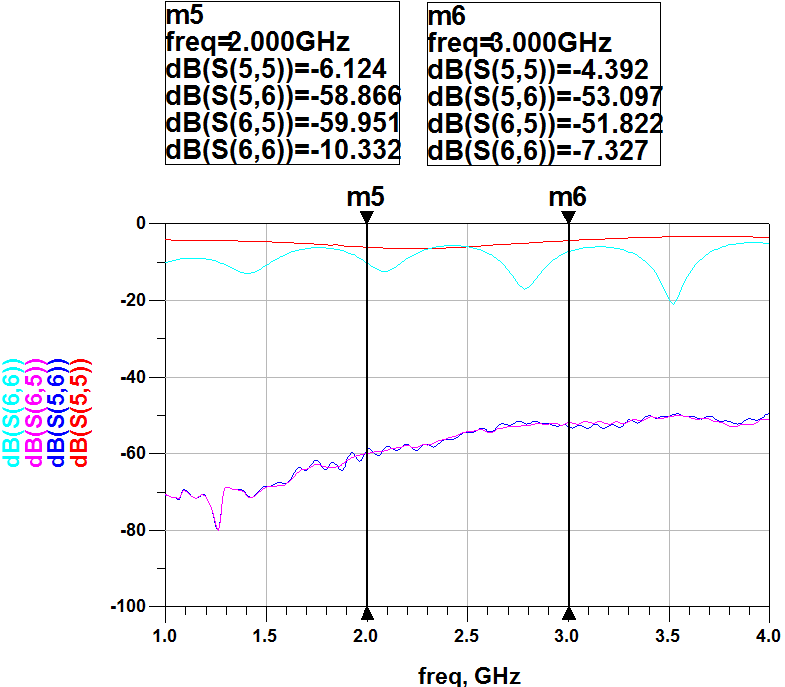
\includegraphics[width=0.75\textwidth]{Design3-3.png}
	\caption{Design 1 S-Parameters - Isolation (Worst case)}
	\label{fig:design1_3}
\end{figure} 
%TODO : S11 input reflection

%TODO : S12 input insertion

%TODO : S21 output insertion

%TODO : S22 output reflection

\subsubsection{Switch Speed}

\subsubsection{Power Requirements}


\subsection{Output 1}
Output 1 has been tested with a VNA, there are $3$ different characteristics that are key to the analysis of the SP16T RF switch: losses, speed and power.

\subsubsection{Losses}
\begin{figure}[H]
	\centering
%	\includegraphics[width=0.75\textwidth]{rf_sparam.png}
	\caption{Output 1 S-Parameters}
	\label{fig:output1_sp}
\end{figure} 
%TODO : S11 input reflection

%TODO : S12 input insertion

%TODO : S21 output insertion

%TODO : S22 output reflection

\subsubsection{Switch Speed}

\subsubsection{Power Requirements}


\subsection{Output 2}		\label{sec:res_out2}
The design for `Output 2' seen in Section \ref{sec:output2} was developed and tested using a VNA; it was found that the design wasn't operating. So due to time constraints, since the RF chip was not functioning it was decided to disregard this design as it would be too expensive and time consuming to re-design \& develop this design.


\subsection{Cabling}		\label{sec:res_cabling}
There are several different cabling options available; three different cabling options have been looked at, this includes flexible and rigid SMA cables, and UFL cabling. Looking at Figure \ref{fig:flex_sma} - \ref{fig:ufl_sma} we can determine the effects of cabling in the final design.
\begin{figure}[H]
	\centering
	\includegraphics[width=0.75\textwidth]{SMA-flex.png}
	\caption{Flexable $0.5$m SMA cable S-Parameters}
	\label{fig:flex_sma}
\end{figure} 
\begin{figure}[H]
	\centering
	\includegraphics[width=0.75\textwidth]{SMA-rig.png}
	\caption{Rigid $0.5$m SMA cable S-Parameters}
	\label{fig:rigid_sma}
\end{figure} 
%TODO : discuss problems with using sma connectors
It can be seen that more rigid cable has a far better response for insertion, although both these cables are particularly bulky in their size. 

\begin{figure}[H]
	\centering
	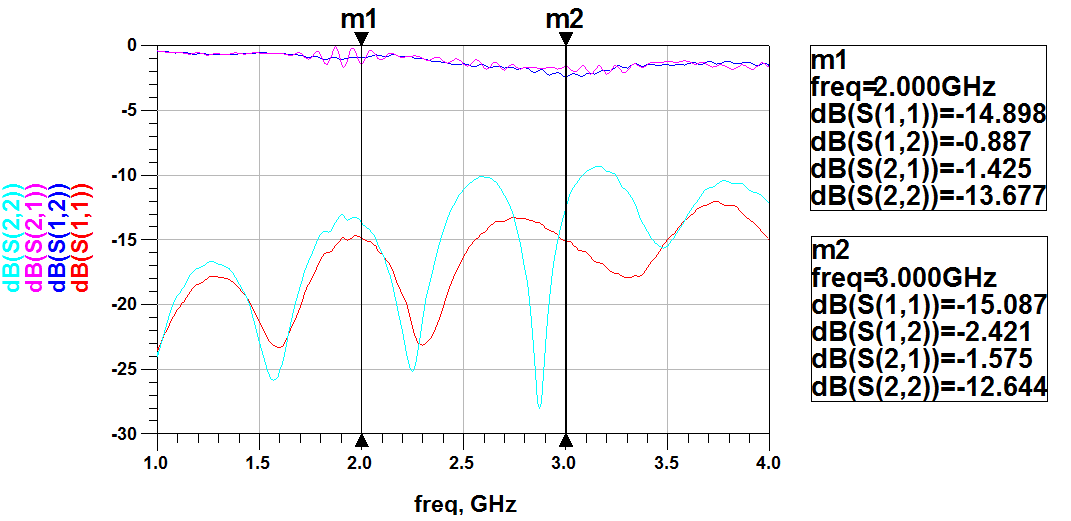
\includegraphics[width=1\textwidth]{UFL-res.png}
	\caption{$0.5$m UFL cable S-Parameters}
	\label{fig:ufl_sma-bad}
\end{figure} 
\begin{figure}[H]
	\centering
	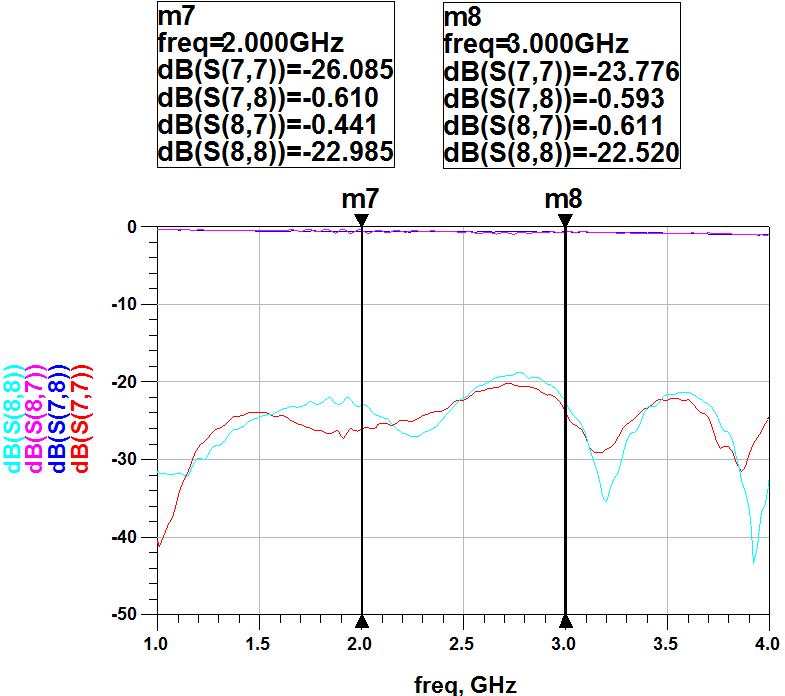
\includegraphics[width=0.75\textwidth]{UFL-short-res.png}
	\caption{$0.5$m UFL cable S-Parameters}
	\label{fig:ufl_sma}
\end{figure} 
It can be seen that there is a larger loss from the UFL cable seen in Figure \ref{fig:ufl_sma} in comparison to the SMA cabling seen in Figure \ref{fig:flex_sma} and \ref{fig:rigid_sma}. It has been decided that the design would suffer this loss in order to allow for a more flexible cabling method allowing for a device which is significantly more portable and smaller. \\
An issue was found that can be seen in Figure \ref{fig:ufl_sma-bad}, this is a UFL connector that has been connected and disconnected multiple times; UFL cabling is commonly designed for less than $20$ mating's. A new UFL cable was tested which can be seen in Figure \ref{fig:ufl_sma}, giving a significantly better response for insertion and reflection.

\section{RF Switch Matrix}
This section looks at the overall characteristics of the final RF switch matrix design. To determine the overall performance of the system, this required evaluating the performance, speed, size and power constraints.

\subsection{Analysis}

\subsection{Final Design}
From looking at the results obtained in Section \ref{sec:indv_boards} it can be seen that the only option for the output SPDT switch is `Output 1'. Therefore the $16$ output terminals will have the reflection seen in Figure \ref{fig:output1_sp} $S_{22}$ signal, this will be connected to the SP16T via a UFL-UFL connector seen in Figure \ref{fig:ufl_sma}. \\
Looking at the results obtained, it can be seen that `Design ...' has an insertion loss of ...dB 

%TODO : finish this section, compare the insertion/isolation between the designs.

Therefore the final design will use  `Design ...' and `Output 1'. 

\subsection{Losses}
In order to determine the characteristics of the designed RF switch matrix, its characteristics of can be modelled using S-Parameters to evaluate the final design. Using the \model \ VNA the switch matrix was analysed to determine the amount of losses that are present in the system. \\
Looking at Figure \ref{fig:rf_sparam} we can determine the performance of the overall system. There are multiple paths that need to be considered in order to fully evaluate the RF switch, there are 9 different paths that can be taken; these can be seen below in Figure \ref{fig:rf_sparam1} - \ref{fig:rf_sparam9}.
%TODO : far to many pictures, only do 3: insertion, isolation best case, isolation worst case

\begin{figure}[H]
	\centering
%    \includegraphics[width=0.75\textwidth]{rf_sparam.png}
	\caption{S-Parameters of RF switch matrix \\ Insertion Loss}
	\label{fig:rf_sparam1}
\end{figure} 
%TODO : S11 input reflection

%TODO : S12 input insertion

%TODO : S21 output insertion

%TODO : S22 output reflection


\begin{figure}[H]
	\centering
%    \includegraphics[width=1\textwidth]{rf_sparam.png}
	\caption{S-Parameters of RF switch matrix\\ Isolation (Best case)}
	\label{fig:rf_sparam2}
\end{figure} 
%TODO : S11 input reflection

%TODO : S12 input isolation

%TODO : S21 output isolation

%TODO : S22 output reflection


\begin{figure}[H]
	\centering
%    \includegraphics[width=0.75\textwidth]{rf_sparam.png}
	\caption{S-Parameters of RF switch matrix\\ Isolation (Worst case)}
	\label{fig:rf_sparam3}
\end{figure} 
%TODO : S11 input reflection

%TODO : S12 input isolation

%TODO : S21 output isolation

%TODO : S22 output reflection




\subsection{Speed}
We know from Section \ref{sec:micro_dev} that micro-controller is capable of controlling the switches at 1500\us , but the SSR's are capable of operating above this speed. Therefore the maximum switching frequency needs to be determined for this RF switch. \\
Using the specifications from the datasheets, it can be said that the maximum switching speed for the switch matrix is 150\us. The 150\us is determined by the slowest chip in this system which bottlenecks the maximum switching speed of the overall performance of the switch matrix. Therefore we can say that theoretical switching speed is limited to .... \us . \\[0.3cm]
With the fully developed RF switch matrix it can be fully evaluated to determine its performance in regard to speed; as can be seen in Figure \ref{fig:speedtest} the switch matrix is wired so that one input and output are connected to the VNA.
\begin{figure}[H]
	\centering
%    \includegraphics[width=0.75\textwidth]{rf_sparam.png}
	\caption{Speed test set-up for RF Switch Matrix}
	\label{fig:speedtest}
\end{figure} 
Using the set-up shown in Figure \ref{fig:speedtest} the VNA monitor's the signal strength to determine the speed which causes the insertion loss to drop bellow the level seen in Figure \ref{fig:rf_sparam1}. By doing this it was determined that the maximum switching speed of the micro-controller is ... \us , which is close to the expected limitation of the ..... RF chip.

\subsection{Power Requirements \& Control}



%---------------------------------------------------------------------------------






%---------------------------------------------------------------------------------
\chapter{Discussion}
\section{Problems}
It was seen that there was a poor reflection in the results from Design 1, Design 3, Output 1 and the final switch matrix; a cause of this poor result is was identified when analysing the cabling in Section \ref{sec:res_cabling}. 

%PROBLEM - Impedance mismatches at io terminals and i/o of chips
%	SOLUTION - Fix trac sizes, add chebyshev transformer at input of chips
%		design alternate transformer
%		Run simulations in ads
%		
\subsection{Impedance Mismatch}	\label{sec:imp-mismatch}

\subsubsection{Simulations}


\subsubsection{Resolving Impedance Mismatch}




\subsection{Resource Availability}



\section{Removing Losses from VNA Results}
Since the loss due to the mismatch discussed in Section \ref{sec:imp-mismatch} can be simulated in ADS as seen in Figure \ref{} we are able to write MATLAB code given in Section \ref{sec:matlab-res}. This MATLAB code de-embeds the S-Parameters of the RF chips from the mismatch caused by the micro-strip track; this result is plotted to estimate the ideal insertion loss and reflection of the switch matrix without the impedance mismatch. 
\begin{figure}[H]
	\centering
%    \includegraphics[width=0.75\textwidth]{rf_sparam.png}
	\caption{Ideal S-Parameters of Switch Matrix}
	\label{fig:ideal-switchmatrix}
\end{figure} 
Therefore it can be seen comparing the results in Figure \ref{fig:ideal-switchmatrix} against the analysed results in Figure \ref{} has improved as the frequency increases. It should be noted that this is not the actual frequency response of a corrected PCB; using ADS a new simulation can be computed to simulated the new loss due to the transmission lines. By adding the S-Parameters 
 of a corrected board without 
 
\begin{figure}[H]
	\centering
%    \includegraphics[width=0.75\textwidth]{rf_sparam.png}
	\caption{Corrected S-Parameters of Switch Matrix}
	\label{fig:corrected-switchmatrix}
\end{figure} 

\subsection{MATLAB Code} \label{sec:matlab-res}
\begin{lstlisting}
asdf
\end{lstlisting}



\section{Objective Fulfilment}


\subsection{Comparison to Available Technology}
%TODO : compare results to the switch relay


\section{Contributions}





%---------------------------------------------------------------------------------









%---------------------------------------------------------------------------------
\chapter{Conclusions and Future Work}

\section{Conclusion}


%TODO : Intergrate an SDR into the switch matrix, replacing the microcontroller allowing for more precise control over switches
%TODO : Resolve impedance mismatch at input/output of switch
\section{Future Work}



%---------------------------------------------------------------------------------




\appendix
\addcontentsline{toc}{part}{Appendices}


\newpage
\chapter{PCB Design}
\section{Design 1}	\label{sec:pcb_design1}

\section{Design 2}	\label{sec:pcb_design2}

\section{Design 3}	\label{sec:pcb_design3}

\section{Output Design 1}	\label{sec:pcb_outdesign1}

\section{Output Design 2}	\label{sec:pcb_outdesign2}

\section{Output Design 3}	\label{sec:pcb_outdesign3}
















\chapter{Substrate Parameters}		\label{sec:substrate_param}
The following tables contain the parameters and details for the substrates investigated in this thesis. \newline
\begin{table}[!htbp]
\centering
\begin{tabular}{L{3cm}C{2cm}C{2cm}}
\hline
Substrate & Parameter & Value \\
\hline
\hline
\multirow{3}{*}{FR-4} & Er & 4.7 	\\
& Mur & 1 \\
& H & even 	\\
\hline
\multirow{3}{*}{Epoxy} & Er & 4.7 	\\
& Mur & 1 \\
& H & even 	\\
\hline
\end{tabular}
\caption{\sl Parameters for simulation of PCB substrate's}
\label{tab:substrate}
\end{table}

\chapter{Bill of Materials}
In order to construct the design of the Switching Matrix we require the following components, a Bill of Materials has been constructed and can be seen in \tab{tab:bom}.
\begin{longtable}{|c|c|c|c|c|c|c|}
\hline
Name & Description & Digikey Part no. & Min Order no. & Price & Quantity & Total \\
\hline
& & & & & & \\
\hline
\multicolumn{7}{c}{} \\
\hline
\multicolumn{5}{|c}{} & \textbf{Total}: & \$$100$\\
\hline
\caption{\sl Bill of Materials}
\label{tab:bom}
\end{longtable}











\chapter{RF Switch Controls}		
\begin{landscape}
\section{Design 1}	\label{sec:logic_design1}
\begin{table}[H]
  \centering
  \caption{`Design 1' Logic Control Table}
    \begin{tabular}{|cccc|ccccccccccccccccccc|}
    \hline
    \multicolumn{4}{|c|}{\textbf{Input}} & \multicolumn{19}{c|}{\textbf{Output}} \\
    \hline
    \multicolumn{1}{|c|}{\multirow{2}[4]{*}{\boldmath{}\textbf{$x_3$}\unboldmath{}}} & \multicolumn{1}{c|}{\multirow{2}[4]{*}{\boldmath{}\textbf{$x_2$}\unboldmath{}}} & \multicolumn{1}{c|}{\multirow{2}[4]{*}{\boldmath{}\textbf{$x_1$}\unboldmath{}}} & \multirow{2}[4]{*}{\boldmath{}\textbf{$x_0$}\unboldmath{}} & \multicolumn{2}{c|}{\textbf{$SPDT_1$}} & \multicolumn{2}{c|}{\textbf{$SPDT_2$}} & \multicolumn{2}{c|}{\textbf{$SPDT_3$}} & \multicolumn{2}{c|}{\textbf{$SPDT_4$}} & \multicolumn{2}{c|}{\textbf{$SPDT_5$}} & \multicolumn{2}{c|}{\textbf{$SPDT_6$}} & \multicolumn{2}{c|}{\textbf{$SPDT_7$}} & \multicolumn{2}{c|}{\textbf{$SPDT_8$}} & \multicolumn{3}{c|}{\textbf{$SP8T$}} \\
\cline{5-23}    \multicolumn{1}{|c|}{} & \multicolumn{1}{c|}{} & \multicolumn{1}{c|}{} &       & \multicolumn{1}{c|}{\textbf{V1}} & \multicolumn{1}{c|}{\textbf{V2}} & \multicolumn{1}{c|}{\textbf{V1}} & \multicolumn{1}{c|}{\textbf{V2}} & \multicolumn{1}{c|}{\textbf{V1}} & \multicolumn{1}{c|}{\textbf{V2}} & \multicolumn{1}{c|}{\textbf{V1}} & \multicolumn{1}{c|}{\textbf{V2}} & \multicolumn{1}{c|}{\textbf{V1}} & \multicolumn{1}{c|}{\textbf{V2}} & \multicolumn{1}{c|}{\textbf{V1}} & \multicolumn{1}{c|}{\textbf{V2}} & \multicolumn{1}{c|}{\textbf{V1}} & \multicolumn{1}{c|}{\textbf{V2}} & \multicolumn{1}{c|}{\textbf{V1}} & \multicolumn{1}{c|}{\textbf{V2}} & \multicolumn{1}{c|}{\textbf{V1}} & \multicolumn{1}{c|}{\textbf{V2}} & \textbf{V3} \\
    \hline
    0     & 0     & 0     & 0     & $x_0$ & $\bar{x_0}$ & $x_0$ & $\bar{x_0}$ & $x_0$ & $\bar{x_0}$ & $x_0$ & $\bar{x_0}$ & $x_0$ & $\bar{x_0}$ & $x_0$ & $\bar{x_0}$ & $x_0$ & $\bar{x_0}$ & $x_0$ & $\bar{x_0}$ & $x_1$ & $x_2$ & $x_3$ \\
    0     & 0     & 0     & 1     & $x_0$ & $\bar{x_0}$ & $x_0$ & $\bar{x_0}$ & $x_0$ & $\bar{x_0}$ & $x_0$ & $\bar{x_0}$ & $x_0$ & $\bar{x_0}$ & $x_0$ & $\bar{x_0}$ & $x_0$ & $\bar{x_0}$ & $x_0$ & $\bar{x_0}$ & $x_1$ & $x_2$ & $x_3$ \\
    0     & 0     & 1     & 0     & $x_0$ & $\bar{x_0}$ & $x_0$ & $\bar{x_0}$ & $x_0$ & $\bar{x_0}$ & $x_0$ & $\bar{x_0}$ & $x_0$ & $\bar{x_0}$ & $x_0$ & $\bar{x_0}$ & $x_0$ & $\bar{x_0}$ & $x_0$ & $\bar{x_0}$ & $x_1$ & $x_2$ & $x_3$ \\
    0     & 0     & 1     & 1     & $x_0$ & $\bar{x_0}$ & $x_0$ & $\bar{x_0}$ & $x_0$ & $\bar{x_0}$ & $x_0$ & $\bar{x_0}$ & $x_0$ & $\bar{x_0}$ & $x_0$ & $\bar{x_0}$ & $x_0$ & $\bar{x_0}$ & $x_0$ & $\bar{x_0}$ & $x_1$ & $x_2$ & $x_3$ \\
    0     & 1     & 0     & 0     & $x_0$ & $\bar{x_0}$ & $x_0$ & $\bar{x_0}$ & $x_0$ & $\bar{x_0}$ & $x_0$ & $\bar{x_0}$ & $x_0$ & $\bar{x_0}$ & $x_0$ & $\bar{x_0}$ & $x_0$ & $\bar{x_0}$ & $x_0$ & $\bar{x_0}$ & $x_1$ & $x_2$ & $x_3$ \\
    0     & 1     & 0     & 1     & $x_0$ & $\bar{x_0}$ & $x_0$ & $\bar{x_0}$ & $x_0$ & $\bar{x_0}$ & $x_0$ & $\bar{x_0}$ & $x_0$ & $\bar{x_0}$ & $x_0$ & $\bar{x_0}$ & $x_0$ & $\bar{x_0}$ & $x_0$ & $\bar{x_0}$ & $x_1$ & $x_2$ & $x_3$ \\
    0     & 1     & 1     & 0     & $x_0$ & $\bar{x_0}$ & $x_0$ & $\bar{x_0}$ & $x_0$ & $\bar{x_0}$ & $x_0$ & $\bar{x_0}$ & $x_0$ & $\bar{x_0}$ & $x_0$ & $\bar{x_0}$ & $x_0$ & $\bar{x_0}$ & $x_0$ & $\bar{x_0}$ & $x_1$ & $x_2$ & $x_3$ \\
    0     & 1     & 1     & 1     & $x_0$ & $\bar{x_0}$ & $x_0$ & $\bar{x_0}$ & $x_0$ & $\bar{x_0}$ & $x_0$ & $\bar{x_0}$ & $x_0$ & $\bar{x_0}$ & $x_0$ & $\bar{x_0}$ & $x_0$ & $\bar{x_0}$ & $x_0$ & $\bar{x_0}$ & $x_1$ & $x_2$ & $x_3$ \\
    1     & 0     & 0     & 0     & $x_0$ & $\bar{x_0}$ & $x_0$ & $\bar{x_0}$ & $x_0$ & $\bar{x_0}$ & $x_0$ & $\bar{x_0}$ & $x_0$ & $\bar{x_0}$ & $x_0$ & $\bar{x_0}$ & $x_0$ & $\bar{x_0}$ & $x_0$ & $\bar{x_0}$ & $x_1$ & $x_2$ & $x_3$ \\
    1     & 0     & 0     & 1     & $x_0$ & $\bar{x_0}$ & $x_0$ & $\bar{x_0}$ & $x_0$ & $\bar{x_0}$ & $x_0$ & $\bar{x_0}$ & $x_0$ & $\bar{x_0}$ & $x_0$ & $\bar{x_0}$ & $x_0$ & $\bar{x_0}$ & $x_0$ & $\bar{x_0}$ & $x_1$ & $x_2$ & $x_3$ \\
    1     & 0     & 1     & 0     & $x_0$ & $\bar{x_0}$ & $x_0$ & $\bar{x_0}$ & $x_0$ & $\bar{x_0}$ & $x_0$ & $\bar{x_0}$ & $x_0$ & $\bar{x_0}$ & $x_0$ & $\bar{x_0}$ & $x_0$ & $\bar{x_0}$ & $x_0$ & $\bar{x_0}$ & $x_1$ & $x_2$ & $x_3$ \\
    1     & 0     & 1     & 1     & $x_0$ & $\bar{x_0}$ & $x_0$ & $\bar{x_0}$ & $x_0$ & $\bar{x_0}$ & $x_0$ & $\bar{x_0}$ & $x_0$ & $\bar{x_0}$ & $x_0$ & $\bar{x_0}$ & $x_0$ & $\bar{x_0}$ & $x_0$ & $\bar{x_0}$ & $x_1$ & $x_2$ & $x_3$ \\
    1     & 1     & 0     & 0     & $x_0$ & $\bar{x_0}$ & $x_0$ & $\bar{x_0}$ & $x_0$ & $\bar{x_0}$ & $x_0$ & $\bar{x_0}$ & $x_0$ & $\bar{x_0}$ & $x_0$ & $\bar{x_0}$ & $x_0$ & $\bar{x_0}$ & $x_0$ & $\bar{x_0}$ & $x_1$ & $x_2$ & $x_3$ \\
    1     & 1     & 0     & 1     & $x_0$ & $\bar{x_0}$ & $x_0$ & $\bar{x_0}$ & $x_0$ & $\bar{x_0}$ & $x_0$ & $\bar{x_0}$ & $x_0$ & $\bar{x_0}$ & $x_0$ & $\bar{x_0}$ & $x_0$ & $\bar{x_0}$ & $x_0$ & $\bar{x_0}$ & $x_1$ & $x_2$ & $x_3$ \\
    1     & 1     & 1     & 0     & $x_0$ & $\bar{x_0}$ & $x_0$ & $\bar{x_0}$ & $x_0$ & $\bar{x_0}$ & $x_0$ & $\bar{x_0}$ & $x_0$ & $\bar{x_0}$ & $x_0$ & $\bar{x_0}$ & $x_0$ & $\bar{x_0}$ & $x_0$ & $\bar{x_0}$ & $x_1$ & $x_2$ & $x_3$ \\
    1     & 1     & 1     & 1     & $x_0$ & $\bar{x_0}$ & $x_0$ & $\bar{x_0}$ & $x_0$ & $\bar{x_0}$ & $x_0$ & $\bar{x_0}$ & $x_0$ & $\bar{x_0}$ & $x_0$ & $\bar{x_0}$ & $x_0$ & $\bar{x_0}$ & $x_0$ & $\bar{x_0}$ & $x_1$ & $x_2$ & $x_3$ \\
    \hline
    \end{tabular}%
  \label{tab:addlabel}%
\end{table}%

\end{landscape}


\subsection{Design 2}




\subsection{Design 3}




\subsection{Output 1}


\subsection{Output 2}






\chapter{Companion disk}

If you wish to make some computer files available to your examiners,
you can list and describe the files here.  The files can be supplied
on a disk and inserted in a pocket fixed to the inside back cover.

The disk will not be needed if you can specify a URL from which the
files can be downloaded.

\cleardoublepage









\addcontentsline{toc}{section}{\protect\numberline{}Bibliography}
\bibliographystyle{IEEEtran}
\bibliography{ref}

\end{document}